\documentclass[]{svjour3}
\RequirePackage{fix-cm}
\usepackage[utf8]{inputenc}
\usepackage[usenames,dvipsnames]{color}
\usepackage{fullpage}

\usepackage[numbers, sort, compress]{natbib}
\usepackage{graphics}
\usepackage{graphicx}
\usepackage{epstopdf}
\usepackage{color}
\usepackage{hyperref}
%\usepackage{pdfsync}
\usepackage{mdwlist}
\usepackage{colortbl}
\begin{document}

\title{Distributed Application Runtime Environment (DARE): A
  Standards-based Middleware Framework For Science Gateways}

\author{Sharath Maddineni \and Joohyun Kim \and Yaakoub El-Khamra \and
  Shantenu Jha}

\institute{Center for Computation and Technology, Louisiana State
  University, \email{jhkim@cct.lsu.edu} \and Center for Computation
  and Technology, Louisiana State University,
  \email{smaddineni@cct.lsu.edu} \and Center for Computation and
  Technology, Louisiana State
  University, % Bioinformatics Laboratory, Academic Medical Center, University of Amsterdam, \email{m.a.santcroos@amc.uva.nl}
  \and Texas Advanced Computing Center, TACC, The University of Texas
  At Austin, \email{yaakoub@tacc.utexas.edu} \and Center for
  Computation and Technology, Louisiana State University, Rutgers
  University, School of Informatics, University of Edinburgh,
  Department of Computer Science, Louisiana State University,
  \email{shantenu.jha@rutgers.edu}}

%\titlerunning{Dynamic Application Runtime Environment (DARE): A Standards-based Framework For Science Gateways}
%\authorrunning{Joohyun Kim et al.}

%\keywords{Science Gateways}
%\subclass{ MSC codes }
%\PACS{ PACS codes }
%\CRclass{ CR codes }

\date{Received: date / Accepted: date}


% \begin{center}
%   Joohyun Kim$^{1}$, Sharath Maddineni$^{1}$, Mark Santcroos$^{1,4}$,
%   Yaakoub El-Khamra$^3$, Shantenu Jha$^{1,2,5,6}$\\
%   $^1$ Center for Computation and Technology, Louisiana State University\\
%   $^2$ Rutgers University
%   $^3$ Texas Advanced Computing Center, TACC, The University of Texas At Austin \\
%   $^4$ Bioinformatics Laboratory, Academic Medical Center, University of Amsterdam\\
%   $^5$ School of Informatics, University of Edinburgh\\
%   $^6$ Department of Computer Science, Louisiana State University\\
% \end{center}


%\numberofauthors{3}
% \author{
% \alignauthor Joohyun Kim\\
%        \affaddr{Center for Computation and Technology}\\
%        \affaddr{Louisiana State University}\\
%        \affaddr{216 Johnston}\\
%        \affaddr{Baton Rouge, LA} \\
%        \email{jhkim@cct.lsu.edu}
% \alignauthor Sharath Maddineni\\
%        \affaddr{Center for Computation and Technology}\\
%        \affaddr{Louisiana State University}\\
%        \affaddr{216 Johnston}\\
%        \affaddr{Baton Rouge, LA}
%        \email{smaddineni@cct.lsu.edu}
% \alignauthor Mark Santcroos\\
%        \affaddr{}\\
%        \affaddr{}\\
%        \affaddr{}\\
%        \affaddr{} \\
%        \email{}
% \alignauthor Yaakoub El-Khamra\\
%        \affaddr{}\\
%        \affaddr{}\\
%        \affaddr{}\\
%        \affaddr{} \\
%        \email{}
% \alignauthor Shantenu Jha 
% \titlenote{Author for correspondence}\\
%       \affaddr{Rutgers University, Piscataway, NJ 08854, US  }\\
%       \affaddr{CCT, Louisiana State University}
% %      \affaddr{214 Johnston}\\
%       \affaddr{Baton Rouge, LA, 70803, US}
%      \email{sjha@cct.lsu.edu}
% }


  % An understanding of challenges and computational requirements of
  % the life-science applications suggests that the uptake of
  % distributed heterogeneous scalable HPC resources demonstrate its
  % effectiveness as an integral component of a wide-range of
  % life-science gateways. DARE science gateways comprise a user
  % access layer and middleware layers built upon Simple API for Grid
  % Application (SAGA) and the SAGA-based Pilot-Job (SAGA-BigJob)
  % capability.
\maketitle

  % However, there are missing capabilities and abstractions that
  % enable the use of the collective capacity of distributed
  % cyberinfrastructure such as TeraGrid/XSEDE, especially those that
  % can be used to develop gateways in an easy, extensible and
  % scalable fashion for both compute and data-intensive applications.

 % However, there are missing capabilities that make distributed
  % cyberinfrastructure such as TeraGrid/XSEDE usable as a
  % collective resource difficult; these missing abstractions include
  % those that can be used to develop Gateways to utilize the
  % collective capacity of distributed cyberinfrastructure in an easy,
  % extensible and scalable fashion for both compute and
  % data-intensive applications.  This is a serious barrier, as
  % Gateways often require customization for specific user groups and
  % infrastructure usage modes.  So whereas a single science gateway
  % is a scalable access mechanism in terms of number of people, that
  % can be supported, the development of multiple similar gateways but
  % with differing infrastructure usage and requirements is not
  % scalable.

% that supports the utilization of distributed resources
%   for both compute and data-intensive applications.


  \begin{abstract}
    Gateways have been able to provide efficient and simplified access
    to distributed and high-performance computing resources. Gateways
    have been shown to support many common and advanced requirements,
    as well as proving successful as a shared access mode to
    production cyberinfrastructure such as the TG/XSEDE.  There are
    two primary challenges in the design of effective and
    broadly-usable gateways: the first revolves around the creation of
    interfaces that catpure existing and future usage modes so as to
    support desired scientific investigation.  The second challenge
    and the focus of this paper, is concerned about the requirement to
    integrate the user-interfaces with computational resources and
    specialized cyberinfrastructure in an interoperable, extensible
    and scalable fashion.  Currently, there does not exist a commonly
    usable middleware to that enables seamless integration of
    different gateways to a range of distributed and high-performance
    infrastructures.  The development of multiple similar gateways
    that can work over a range of production cyberinfrastructures,
    usage modes and application requirements is not scalable without a
    effective and extensible middleware.  Some of the challenges that
    make using production cyberinfrastructure as a collective resource
    difficult are also responsible for the absence of middleware that
    enables multiple gateways to utilize the collective
    capabilities. We introduce the SAGA-based, Distributed Application
    Runtime Environment (DARE) framework, using which gateways that
    seamlessly and effectively utilize scalable distributed
    infrastructure can be built.  We discuss the architecture of
    DARE-based gateways, and show using several different prototypes
    -- DARE-HTHP, DARE-NGS, how gateways can be constructed by
    utilizing the DARE middleware framework.
\end{abstract}

%  This work is predicated on three important trends: (i) that the
%   importance, impact and percentage of TeraGrid/XSEDE resources
%   assigned to the life sciences is increasing at a rate that is
%   probably greater than other disciplines, (ii) that gateways have
%   proven to be a very effective access mechanism to distributed HPC
%   resources provided by the TeraGrid/XSEDE, and in particular a very
%   successful model for shared/community access models, and (iii) that
%   in spite of the previous two points there are missing capabilities
%   and abstractions that enable the use of the collective capacity of
%   distributed cyberinfrastructure such as TeraGrid/XSEDE, especially
%   those that can be used to develop gateways in an easy, extensible
%   and scalable fashion for both compute and data-intensive
%   applications. We introduce the SAGA-based, Dynamic Application
%   Runtime Environment (DARE) framework from which extensible,
%   versatile and effective gateways that seamlessly utilize scalable
%   infrastructure can be built for a life-science applications. We
%   discuss the architecture of DARE-based gateways, and particularly
%   life-science gateways -- DARE-HTHP, DARE-NGS, DARFOLDFOLD, and
%   DARE-DOCK, that use the DARE-framework to support a wide-range of
%   life-science capabilities.


\newif\ifdraft
\drafttrue                                                                                        \
\ifdraft
 %\newcommand{\reviewer}[1]{ {\textcolor{blue}    { ***Reviewer:     #1 }}}
 \newcommand{\jkimnote}[1]{{\textcolor{green}   { ***Joohyun:   #1 }}}
 \newcommand{\jhanote}[1]{  {\textcolor{red}     { ***SJ: #1 }}}
  \newcommand{\smnote}[1]{  {\textcolor{red}     { ***Sharath: #1 }}}
 \newcommand{\todo}[1]{  {\textcolor{red}     { ***TODO: #1 }}}
 \newcommand{\fix}[1]{  {\textcolor{red}     { ***FIX: #1 }}}
\newcommand{\yyenote}[1]{  {\textcolor{blue}     { ***YYE: #1 }}}
 \newcommand{\reviewer}[1]{}
\else
 \newcommand{\reviewer}[1]{}
 \newcommand{\yyenote}[1]{}
 \newcommand{\jkimnote}[1]{}
 \newcommand{\smnote}[1]{}
 \newcommand{\jhanote}[1]{}
 \newcommand{\todo}[1]{  {\textcolor{red}     { ***TODO: #1 }}}
 \newcommand{\fix}[1]{}                                                                              
 \fi



% \category{D.1.3}{Software}{Concurrent Programming}{ Distributed programming/parallel programming} 
% \category{J.3}{Computer Applications}{Bioinformatics}

% \section*{General Terms}{Design,Measurement,Theory}

%  \keywords{Science Gateway, Runtime Environment, Distributed Computing, Simple API for Grid
%   Applications (SAGA), Pilot-Job abstraction, Data-intensive Computing}

\section{Introduction}


% as seen from Figs.~\ref{tg2007} \& \ref{tg2008} and
% Table~\ref{tg2011}, the trends are somewhat unambiguous: among
% consumed computing resources via TeraGrid (TG), now XSEDE, the
% NSF-funded nationwide Cyberinfrastructure (CI) started in 2001 and
% operated between 2004 and 2011 in the USA, the percentage devoted to
% the life sciences is already more than any discipline and the usage
% seems to be increasing, whether measured by number of cycles consumed,
% users or allocations~

% The single largest community is the life-sciences community --
% including MD (25\%)... Get a break-down of the total usage of the TG
% by discipline and application type.


% due to the as well as the advent of computing power and data
% management capacity.

% and consequent challenges arises in the context of Next-Generation DNA
% Sequencing (NGS) technologies, with unprecedented amounts of data
% produced through high-throughput methods and increasing computational
% requirements for gathering, management, and the analysis of associated
% or produced data sets along a pipeline process.

 
% However, most life-science applications have not been very effective
% in utilizing HPC cyberinfrastructure.

% Commented out by yye00, figure is referenced in a paragraph that has been commented out
% \begin{figure}
%  \centering
% 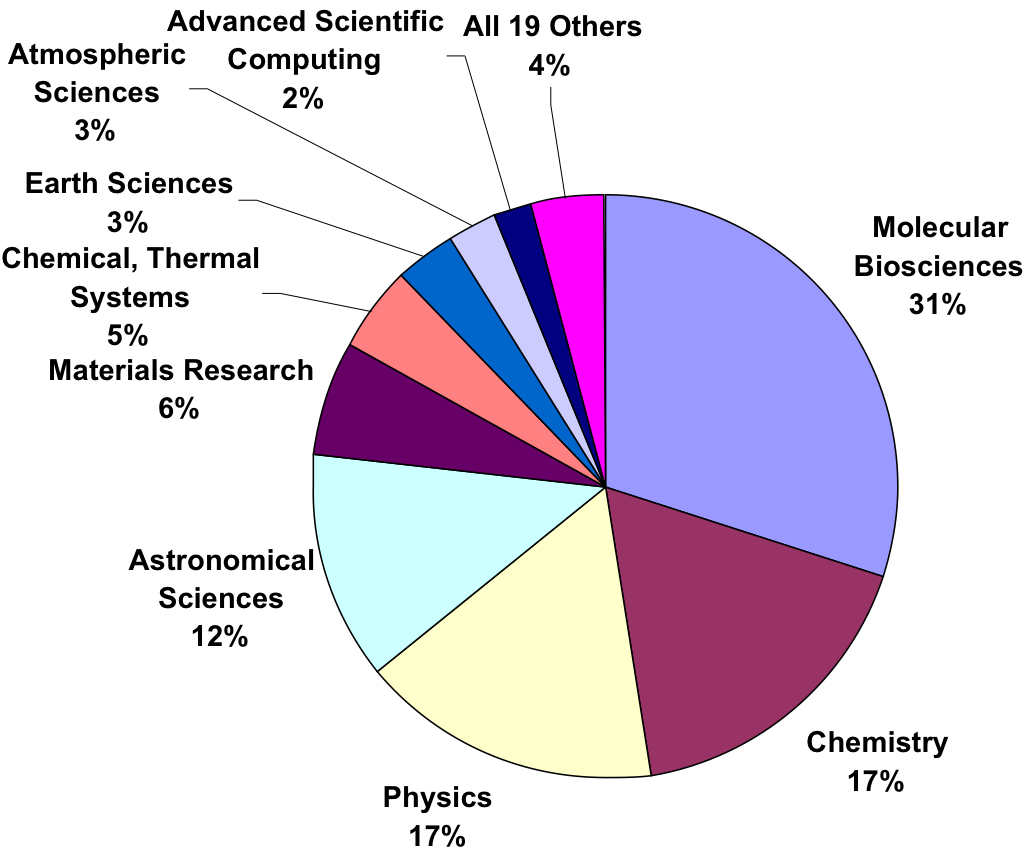
\includegraphics[scale=0.40]{figures/teragrid-discipline07}
% \caption{\small 2007 Usage statistics for the TG. (Reference
%   \url{http://www.teragridforum.org/mediawiki/images/9/90/II_WorkShop_G-HPC_Nework_2009-Towns.pdf})}
%   \label{tg2007}
% \end{figure}


% MD simulations have mostly relied on scaling-up to high core-counts,
% whilst virtual docking calculations benefits from high-throughput
% calculations.  with the exception of a few common applications,
% e.g., large-scale simulations (mostly Molecular Dynamics(MD)) and
% virtual-docking simulations,


% represents a case that

% for analyzing large volumes of data are
% effectively managed.

% required data analytics required
% along with dealing with 

%A specific example highlighting these trends and consequent challenges

Science Gateways have witnessed impressive achievements in terms of
the growth of the number of supporting researchers and computing time
usages~\cite{gce11-nancy}. According to the very recent report about
TG/XSEDE Science Gateway program~\cite{gce11-nancy}, whereas, in 2006,
10 gateways consumed 100,000 CPU hours, in 2010, 22 gateways provided
40 million hours usage; by 2011 nearly 40\% of users on TG/XSEDE came
through TG/XSEDE gateways. Interestingly, the CIPRES phylogenetic
gateway, which was notably absent a few years ago, accounts for 25 \%
of all TG/XSEDE users in 2011. Such rapid and broad uptake of
gateways, is indicative of their potential of supporting existing and
novel scientific computing practices and consequently for advancing
associated scientific domains.

%  exceeding other gateways dedicated to
% traditionally large-scale scientific computing domains, indicating a
% great potential of the gateway development for nurturing novel
% scientific computing practices and consequently for advancing
% associated scientific domains.
 

% Based on the usage of the TG/XSEDE Science Gateways in first quarter
% of 20011, 3-4 of $\approx$ 20 TG/XSEDE gateways currently are
% biological/life science, which in turn account for about $\approx$
% 35\% of all gateway cycles used. Helped by the aforementioned four
% gateways, although existing life-science gateways account for a
% significant fraction of all gateway cycles usage, access to TG/XSEDE
% via gateways accounts for only %2-3\% of
% a fraction of all cycles devoted to biosciences
% %all cycles used, even though molecular biosciences
% (which by most accounts represented 25\% of TG/XSEDE (NU) cycles used
% in Q1-2011.~

Based on the usage of the TG/XSEDE Science Gateways in first quarter
of 2011, gateways catering to biological/life sciences account for
$\approx$ 35\% of all cycles accessed via gateways.  On the
other hand, access to TG/XSEDE via gateways accounts for only a
fraction of all cycles devoted to biological/life sciences, which by
most accounts represented 25\% of TG/XSEDE (NU) cycles used in
Q1-2011\footnote{It is difficult to provide such information in a
  consistent way as the total number of cycles available year-to-year
  varies, but also which discipline a proposal gets assigned to is
  somewhat random; thus many chemistry proposals, even physics
  proposals are likely to be biological in nature. Also, although we
  are referring to life-science applications in general information is
  provided under bio-molecular bio-sciences which are understood to
  represent a large fraction of computational life-science
  applications.}.  

Additionally, although a significant fraction of the biological/life
sciences TG/XSEDE cycles are devoted to molecular biosciences, of
which MD is the dominant component, only a few of the MD users
actually use gateways to access TG/XSEDE resources. Thus, by most accounts
at best only 10\% of all life-science applications cycles are accessed
via gateways.  % Additionally, the dominant growth in computing is
% coming from novel application areas such as NGS which can benefit from
% community provided gateways.
Thus given the overall success and uptake of the gateways approach,
{\it prima facie} there are reasons to believe that if a scalable,
effective and extensible capability were provided for life-science
applications, this {\it gap} could be overcome.

% However, these 4 gateways account
% for about 2-3\% of recording molecular bioscience usage.
%  by some
% accounts representing 25\% of TG/XSEDE~\footnote{It is difficult to
%   provide such information in a consistent way as the total number of
%   cycles available year-to-year varies, but also which discipline a
%   proposal gets assigned to is somewhat random; thus many chemistry
%   proposals, even physics proposals are likely to be biological in
%   nature.}  (NU) cycles used in Q1-2011,

 
% Commented out by yye00, paragraph where this is used has been commented out
% \begin{figure}
%  \centering
% 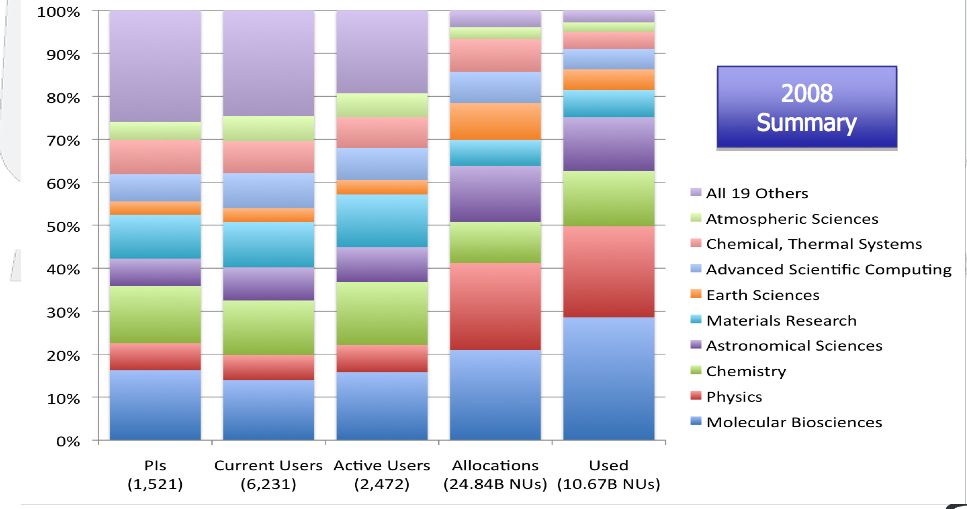
\includegraphics[scale=0.27]{figures/teragrid-discipline08}
% \caption{\small 2008 Usage statistics for the TG/XSEDE (Reference
%   \url{http://www.teragridforum.org/mediawiki/images/d/d8/DEISA-PRACE-May2009-Towns.pdf})}
%   \label{tg2008}
% \end{figure}

The cyberinfrastructure (CI) considerations required to support a
broad-range of analytical approaches and at the scales required, has
received less attention than the data-management problem and
algorithmic advances. Thus not surprisingly, traditional production
cyberinfrastructure, such as the TG/XSEDE, have not been used for such
data-intensive analytics and distributed applications. There are
multiple reasons, but a few contributing factors are: (i) insufficient
runtime environments to support concurrent execution, (ii) historical
emphasis on a separation of compute-intensive and data-intensive
computing, whereas in practice interfaces, tools and abstractions that
support analytics that require both concurrently, i.e., providing
large-scale computational capabilities that work with large-data sets
in an easy, scalable and extensible fashion, (iii) insufficient
support for user-customizable and extensible ``workflows'' that
effectively hide the challenges of data-movement and efficient
data-management whilst managing concurrent distributed (computational)
resources.

The potential advantage of providing gateways for life-science
applications presents a strategic opportunity.  Reconciling the
opportunity, with missing capabilities to support existing and
emerging science gateways (e.g., data-intensive applications) to
utilize distributed cyberinfrastructure in a scalable and extensible
fashion provides the motivation for our work: to develop a simple,
extensible middleware which can be used to stand-up gateways for the
life-sciences so as to utilize distributed and high-performance
cyberinfrastructure. \jhanote{Although initially motivated by
  life-sciences applications, the techniques and abstractions are
  widely applicable.}

% {\it Towards a common middleware for Gateways:} A fundamental design
% objective of Science Gateways is to capture the common requirements of
% the science scenarios, make it easy to support their computational
% requirements, whilst providing the right abstractions to support them
% and making the application/usage-mode specific parts easy to support.
% This objective imposes an important constraint and requirement on the
% tools \& frameworks used to develop Science Gateways.

% to enable/facilitate/support them by making the application/usage-mode
% specific parts easy to support.
%it aims to enable and to provide

%{\it Towards a common middleware for Gateways:}
A fundamental design
objective of Science Gateways is to capture and support common
requirements of the science scenarios, and to support them in a simple
and extensible fashion by providing the right abstractions.  Building
effective science gateways has two major tracks: the first is the
development of effective interfaces and tools that capture application
requirements, e.g., expression of workflows etc, and making these
accessible via community/shared accounts with proper security and
credentials supported. These must be customizable and extensible to
the end-user communities need and specific scientific
requirements. The second is the integration of these interface/tools
with a broad range of high-performance and distributed computational
(HPDC) infrastructure to support the science requirement, but in a way
that is scalable and flexible.  It is important to separate these
challenges, both conceptually and in practice.  This objective imposes
important requirements on the middleware, tools and frameworks used to
develop Science Gateways.

Many gateway development efforts use development
frameworks such as the Open Grid Computing
Environments\cite{ogce-2010} (OGCE); however development frameworks
such as OGCE do not support the integration with the underlying HPDC
infrastructure, i.e., most gateways still enforce the tight-coupling
between applications and a specific infrastructure (see
table~\ref{table:TG-sg}), without support for flexible distributed
execution.  A primary reason is the additional and significant
complexity in %providing the right abstractions so as to enable an
enabling applications to seamlessly utilize distributed
cyberinfrastructure. Such requirements become harder to meet as the
number of connected sites and heterogeneity grows. Interestingly, both
the TG in its transition to eXtreme Science and Engineering Discovery
Environment (XSEDE)~\cite{XSEDE} and EGEE in its transition to EGI
increased the number of middleware distributions they ``support''.
XSEDE supports globus, UNICORE and GENESIS; EGI supports gLite,
Globus, ARC and UNICORE.

% seamlessly transform a target application to be able to seamlessly ,
% and thus into a distributed application.

% as well as the computing power and the data storage capacity of each
% resource reach peta or exa scales.

\begin{table}
\centering
 \small
\begin{tabular}{|c|c|c|c|c|c|} 
  \hline  Quarter & PIs & Current & Active & Allocations  & Usage\\
  & & Users  &  Users & (NUs) $\times 10^6$& (NUs) $\times 10^6$ \\ \hline
  Q3 2010 & 249 & 1,044 & 366 & 8,810   & 2,219  \\ \hline
  Q4 2010 & 254 & 1,040 & 356 & 11,720  & 2,658, \\ \hline
  Q1 2011 & 257 & 1,168 & 418 & 13,101  & 3,412\\ \hline 
\end{tabular} 
\caption{Life-Science usage of the TG/XSEDE over the recent
  quarters. The figures establish that both the  allocation and the
  usage of life-science applications is increasing at least in
  proportion to the increasing resource availability on the TG/XSEDE,
  if not faster.}
 \label{tg2011} 
\end{table}


%\jhanote{Need to discuss}


% which is often eased by the development of a framework.  More
% importantly, supporting a \jhanote{need to define? why should the
%   reader care?}  is critical considering different application usage
% modes for different life-science applications.  \yyenote{The
%   following is a confusing sentence}\jkimnote{I tried to change it}

Viewed from a different perspective, there are difficult challenges (i.e.,
integrating with heterogeneous HPDC infrastructure) and there are
application/usage scenario specific challenges in building science gateways. The
contribution of this work is to address the former challenge via the
development of middleware for Gateways so as to support the effective
integration of these two different tracks.
%, viz., enable different
%application-specific UIs (and security contexts) to utilize a range of
%high-performance and distributed computational (HPDC) infrastructure.

The role of effective middleware is to support maximum reusability in
integrating with HPDC infrastructure. For example, it is always
challenging to integrate new applications, to implement distributed
data management with newly added infrastructure, whilst supporting
existing and novel execution patterns; any framework that aims to
facilitate integration with HPDC infrastructure must also address
these challenges.  Thus any framework used to build science gateways
that provides simple and scalable integration with the HPDC
infrastructure must support broad range of diverse execution patterns
(i.e., commonly occurring modes of using HPDC infrastructure).

%Specifically, we address the following problem: Although Science
%Gateways have proven to be very effective access mechanisms to
%distributed HPC resources provided by the production
%cyberinfrastructure such as TeraGrid/XSEDE and in particular a very
%successful model for shared/community access models, however, there
%are missing capabilities and abstractions that enable the use of the
%collective capacity of distributed cyberinfrastructure such as
%TeraGrid/XSEDE, especially those that can be used to develop a range
%of functionally similar yet slight different gateways in an easy,
%extensible and scalable fashion for both compute and data-intensive
%applications.

% As shown in Table~\ref{table:four-applications},
% flexible execution/usage of four life-science applications are
% summarized by contrasting conventional versus distributed modes.


% \yyenote{The following is the same incredibly long 3 sentences rolled into 1 from the abstract. Needs a bit of change}

% This work is predicated on three important trends: (i) that the
% importance, impact and percentage of TG/XSEDE resources assigned to the
% life sciences is increasing at a rate that is probably greater than
% other disciplines, (ii) that gateways have proven to be a very
% effective access mechanism to distributed HPC resources provided by
% the TG/XSEDE (and in particular a very successful model for
% shared/community access models); given the landscape of the future
% distributed cyberinfrastructure, we anticipate the importance of
% gateways will continue to increase, and (iii) that there are missing
% capabilities and abstractions to enable the use of the collective
% capacity of distributed cyberinfrastructure such as TG/XSEDE, especially
% those that can be used to develop gateways in an easy, extensible and
% scalable fashion for both compute-intensive and data-intensive
% applications.


% gateway development concentrates on the
% development of a runtime environment for distributed applications. T

We introduce the Distributed Application Runtime Environment (DARE)
framework; we illustrate and demonstrate the development of a runtime
environment that supports as a primary design objective the
distributed execution of applications on HPDC infrastructure.  In
general, DARE supports the general goals of distributed applications:
interoperability, dynamic execution %distributed scale-out,
extensibility, adaptivity, scalability (scale-up, scale-out and
scale-across) -- referred to as IDEAS~\cite{ideas}.  DARE builds upon
and utilizes SAGA to achieve the IDEAS objective.  {\it Scale-up} --
or the most common type of scaling behavior, refers to the need of a
single simulations of using many cores efficiently; {\it Scale-out} is
a measure of the ability to support the concurrent execution and
management of multiple tasks/jobs respectively (either on a single
resource, or across multiple physically distributed resources); {\it
  Scale-across} is raised by the need to efficiently distribute across
multiple distinct and possibly heterogeneous resources. {\it
  Adaptivity} addresses the requirement that distributed applications
may have to adapt to resource fluctuation across platforms, and to the
availability of dynamic data.

\begin{table}
\centering
 \small
\begin{tabular}{|c|c|c|c|} 
  \hline Gateway  & Science & Infrastructure & Execution Mode 
  \\
  Name & Domain & Used & \\ 
  &  &  & \\
  & & & \\  \hline \hline 
  
  CIPRES   & phylogeny  &  single node  & multiple  \\
   &  &   & independent   \\ 
  &  &  &  tasks \\  \hline
  GridChem   & quantum & single node or     & multiple  \\
     & chemistry, & small cluster & independent   \\
  & MD &  & task  \\ \hline
   GridAMP     & ASTEC  & legacy domain  & pipelined \\ 
  & coupled with  &  scientific code   & HPC  \\
  & a parallel GE &   &  programs \\ \hline
  Nano  & portal  & large set   & multiple \\
  Hub  & for nano- & of tools  & independent \\
   & technology &  & tasks \\ \hline
  \hline
\end{tabular} \caption{Examples of existing TG/XSEDE Science Gateways. The list is not necessarily complete. More information including URLs can be found elsewhere \cite{tg-sg-list-url}. ASTEC means Aarhus Stellar Evolution Code.}
 \label{table:TG-sg} 
\end{table}

Before we introduce the DARE framework we discuss the ``D'' in
DARE. Although the ``D'' is for Distributed, a fundamental attribute
of many applications -- distributed or otherwise, and infrastructure
that DARE is designed to support is that of ``dynamism''.  Dynamic
aspects come from both an understanding of applications/analytical
requirements, as well the runtime/infrastructure characteristics.  The
fact that application configurations can change as a consequence of
the results produced, or the analytical requirements often means that
minor changes in the application (runtime) properties/results often
lead to large differences in the HPDC infrastructural requirements,
duration of runs etc. The HPDC infrastructure utilized often varies,
and thus runtime decisions related to scheduling and resource
aggregation need to be made. DARE provides fundamental support for
such dynamic execution via pilot-jobs, in particular the SAGA-based
pilot-job (BigJob).

%\yyenote{Insert pilot job definition here. Moved reference}

Pilot-jobs provide a simple approach for decoupling workload
management and resource assignment/scheduling, via the concept of
utilizing a placeholder job as a container for a set of compute tasks.
They thus provide an effective abstraction for dynamic execution and
resource utilization in a distributed context.
Pilot-Jobs~\cite{pstar12} have been shown to be an excellent
abstraction for supporting dynamic/runtime resource allocation and
selection.  In fact, there are reasons to expect Pilot-Jobs as an
excellent abstraction to support the formulation of dynamic
applications as well~\cite{pstar12}. Pilot-Jobs are particularly well
suited for distributed environments.  We have shown that a flexible
Pilot-Job framework can provide the ability to run many MD simulations
effectively across multiple resources on the
TG/XSEDE~\cite{saga-royalsoc,saga_bigjob_condor_cloud}.  Specifically,
we've shown how a SAGA-based implementation of the pilot-job, supports
the distributed application design objectives categorized by the term
IDEAS\cite{ideas}.

It is important to establish the relationship between DARE, BigJob and
SAGA.  In order to do so, we first examine the relationship between
pilot-jobs and SAGA: BigJob is a pilot-job framework that uses the
SAGA API to manage files and job submission to distributed
resources. DARE uses BigJob -- the SAGA based pilot-job as the primary
execution environment for tasks assigned to it. Specifically, DARE
extends and provides BigJob capability (and pilot-jobs in general) for
pre-determined and customized applications using two possible routes:
(i) via templatized support for execution patterns (such as
abstract pipelines specifying dependencies and the order of
execution), or (ii) via pre-defined interactions between tasks.
 
As we will discuss in the next section, the DARE framework makes
extensive use of Pilot-Jobs and is also designed to support
distributed and dynamic applications as a primary/fundamental
attribute.  In this paper we establish how these capabilities can be
generalized to a range of applications via an extensible and
interoperable framework and provided via Science Gateways, to support
a range of life-science applications.  The validation of DARE lies in
establishing its effectiveness as an integral component for multiple
life-science gateways, and by demonstrating that it can enable the
utilization of the collective capabilities of distributed
cyberinfrastructure such as the TG/XSEDE and LONI in a simple and
extensible fashion for a range of life-science applications.

In \S2 we provide background information on SAGA, SAGA-based
pilot-jobs and the need/role for a standards-based building block that
can be used by a range of Science Gateways.  A primary contribution of
this work is to address the latter need via design and implementation
of the DARE framework.  It is important to distinguish DARE from
DARE-based Gateways: DARE is SAGA-based framework that supports
different abstractions such as Pilot-Jobs which in turn are packaged
and integrated with support for other capabilities, such as execution
pattern (e.g. MapReduce, M-W etc). A DARE-based Gateway is one that
uses the DARE framework to implement the coupling to HPDC
infrastructure for a scientific gateway.  \S3 discuss DARE and the
four layered architecture of DARE-based Gateways. In \S4 we present
examples of DARE-based Gateways that we have been developing, followed
by a discussion of the novel deployment models for DARE-based Gateways
on XSEDE. We also discuss data-management support within the DARE
framework.

\jhanote{Need to talk about LifeScience Applications on OSG and EGI,
  i.e., generalise from XSEDE}

% \jhanote{Should we bring this down to two?}

\begin{table}
\centering
 \small
\begin{tabular}{|c|c|c|c|} 
  \hline Science  & Supported  & Conventional   &   Distributed
  \\
  Domain & Applications & Usage Mode & Usage Mode\\ \hline \hline 
% &  cation(s) & & \\  
  
  Molecular   &  \texttt{NAMD} &  MPI-based  & ensemble-based   \\
  Dynamics  &  & single simulation  & multiple  \\ 
  &  & run &  simulation  \\ 
  &  &  &  runs \\ \hline
    NGS data     &  \texttt{BFAST} & memory-intensive  & data-intensive\\ 
  analytics  &  &  single-node   &  distributed  \\
  & & execution  & computing \\ \hline
    \hline
\end{tabular} \caption{Examples of life-science applications of
  interest and their usage modes.  Gateways were developed for these
  applications using the DARE framework \jhanote{I would say we
    provide non-DARE LS examples here!}}
 \label{table:four-applications} 
\end{table}

%no sign to see the end of influx of new tools considering continuous 

%\textit{RNA structure prediction and beyond:} Defying the old
%biological dogma, positioning RNAs as a genome information
%intermediate between DNAs and proteins, during the last couple of
%decades, the number of scientific observations found that RNAs were
%actively involved significantly in gene expression and
%regulation\cite{joyce1999}. %,amaral2008}.
%Now, with the well-known categories of non-coding RNAs such as miRNAs
%and riboswitches, in spite of their biogenesis that does not need to
%be translated into proteins, significant roles of RNAs are quite well
%recognized\cite{costa2009}.
%%ellington2007}. 
%Importantly, RNA functions by forming required structure(s), and the
%pattern of structure formation of RNAs are somewhat contrasted to
%proteins that are mostly folded into highly specific 3-D
%structure\cite{roth2009}. For example, riboswitches chose one of two
%alternative structures, in response to metabolite binding,
%consequently resulting in two different gene regulation stages, i.e.,
%turning on downstream gene synthesis or turning it
%off\cite{montange2008}. Therefore, RNA structure prediction has been
%the major area for RNA studies and noticeable progress was made
%recently for RNA 2D structure prediction as well as 3D structure
%modeling\cite{shapiro2007}.
%
%\textit{Drug Discovery via Virtual Screening strategies:} For small
%molecule drug discovery, virtual screening using a docking method has
%been widely utilized and an immediate requirement for massive docking
%calculations against a chemical database has been attempted by
%managing such many tasks using a local cluster, HPC cluster, grids,
%and clouds\cite{levesque2009,yim2010}. The nature of required
%application usage mode for virtual screening methods is a generic
%example of many task computing, implying that pleasingly parallel
%massive tasks carrying out a docking computation should be executed.
%In spite of such well-established protocol, the challenges in drug
%discovery finding putative inhibitors for target receptors are not
%resolved due to intrinsic difficulties with underlying
%physico-chemical models associated with the issues with scoring
%function, receptor flexibility, and docking strategy itself.
%Therefore, more computing power and scaled calculations by varying the
%parameters for virtual screening are needed in order to understand the
%accuracy of results, suggesting the need of scalable infrastructure is
%highly appreciated while the application usage mode is generally
%intact.

% \subsection{Computational requirements and challenges}

% A growing limitation of applications in the life sciences is that
% workflow, data management, and analysis have become rate limiting
% steps: what is missing is support for the end-to-end execution
% requirement of applications.

% In essence, the move from executing an individual task to
% \textit{large ensembles} of coupled/loosely/uncoupled tasks requires
% scientists to spend significant time on compute and data management
% problems, instead of core science. The quantitative shift (massive
% distributed parallel compute and data resources) implies qualitative
% change in the way how life-science applications are being served for
% scientific discovery.

% We also need to move to tiered sets of computational resources. For
% example, one can imagine running large ensembles of MD engines on
% tightly coupled parallel machines (like Ranger or Kraken) with
% real-time data streamed to separately running analysis and
% visualization resources (Lonestar, Spur), with on-the-fly monitoring
% to analyze convergence, interesting phenomena or problems. This also
% provides the means for possible steering, for example by spawning or
% stopping separate elements of the ensemble to sample more or less in a
% particular region of interest. In addition to real time monitoring,
% hidden correlations in the data require the saving of coarser grained
% simulation data on longer term (1-2 year) disk resources for further
% analysis and mining using less tightly coupled computational
% resources, and ultimately placing reduced and derived data sets
% seamlessly back to the campuses, archivers, and for public
% distribution. Not only does this support the need for diverse sets of
% computational resources, large-scale storage and data transfer
% requirements for sophisticated analysis and visualization, and
% high-bandwidth networking, it also drives the need for software tools
% that facilitate the complicated workflow management, that allow
% dynamic monitoring, starting and stopping of ensemble elements without
% losing access to the global communications fabric and local
% connections, and that provide the means for facilitating data
% management and analysis.

% In essence, the move from executing an individual task to
% \textit{large ensembles} of coupled/loosely/uncoupled tasks requires
% scientists to spend significant time on compute and data management
% problems, instead of core science. The quantitative shift (massive
% distributed parallel compute and data resources) implies qualitative
% change in the way how life-science applications are being served for
% scientific discovery.

% The quantitative shift (massive
% distributed parallel compute and data resources) implies qualitative
% change in the way how life-science applications are being served for
% scientific discovery.

% \section{DYNAMIC APPLICATION RUNTIME ENVIRONMENT (DARE)}
%\subsection{Pilot-Jobs for Life-Sciences For Distributed Applications}
%\jhanote{SJ}

% Pilot-jobs are about the separation of resource assignment and
% workload management.


%\section{DARE: A Runtime Environment for Distributed Applications}\\

% \section{DARE: Standard-based Framework for Distributed Applications
%   Development and Runtime}


\section{DARE: Standard-based Middleware Framework for Science
  Gateways}

%\jhanote{Explain why we call it a Middleware Framework}

In the introduction we outlined the first of two major tracks for
building effective science gateways: the development of effective user
interfaces and associated tools that capture application requirements
(e.g. expression of workflows).  The UI must be customizable and
extensible to meet the specific scientific requirements of different
end-user communities.  The second is the use of HPDC infrastructure in
a scalable and flexible fashion to support as many different
applications and workflows as possible.  Combining the two, it becomes
the role of science gateway middleware to support effective
integration of different application-specific UI tools with underlying
HPDC infrastructure. Successful integration would thus result in
end-user communities customising base-capabilities with low overhead
that meet science requirements and can utilize a range of HPDC
infrastrucutre.

Currently science gateway development requires scientists and
developers to spend non-trivial amounts of time resolving everything
from job submission script errors to data management problems. Simple
as it sounds, to the best of our knowledge, there does not exist
middleware capabilities that provide the ability to utilize different
HPDC infrastructure, using a single, simple API, whilst supporting a
range of application/web development frameworks.  To address these
issues, and to provide a basis for rapid science gateway development
that is capable of utilizing HPDC resource, the DARE~\cite{dareurl}
middleware framework, hereafter referred to as the DARE, has been
developed.

Many of the critical features of the DARE framework are provided by
SAGA and the Pilot-Job capability:
SAGA-BigJob~\cite{saga_bigjob_condor_cloud}.  The SAGA components
provide the distributed capabilities such as remote job submission and
data movement across machines (including data archiving).  A
integrated layer above the resource management layer, provide the
ability to support dynamic execution patterns and workflows.  
DARE allows gateway developers and scientists to focus on the unique
requirements of their scientific applications, as opposed to focus on
the ``plumbing'' of using HPDC infrastructure as well as making it
easier to support application-level constructs, e.g., how to submit
ensembles of simulations to several supercomputers concurrently and
archive their results.

% Using
% SAGA and SAGA-based frameworks to build science gateways meets a
% fundamental design objective of IDEAS~\cite{ideas} (Interoperability,
% Dynamic Execution, Extensibility, Adaptive/Autonomic and Scalability).

 
% DARE is flexible by design, it can be used to support dynamic
% execution of simple stand-alone applications or more complex
% distributed workflows on HPDC infrastructures. Details of science
% gateway building using DARE are explored in \S3.

\subsection{SAGA: Standards-based Access to the Resources Layer}

The Simple API for Grid Applications (SAGA)~\cite{saga_url} is an
implementation of an Open Grid Forum (OGF) Technical Specification
that provides a common and consistent high-level API for the most
commonly required functionality to construct distributed
applications. It also provides a high-level
API~\ref{fig:saga-overview} to construct tools and frameworks to
support distributed applications. The functional areas that are
supported by SAGA include job-submission, file transfer and access, as
well as support for data streaming and distributed coordination.  SAGA
provides both a syntactic and semantic unification via a single
interface to access multiple, semantically distinct middleware
distributions.

Key advantages to development using SAGA include, but are not limited to:
(i) providing a general-purpose, commonly used yet standardized functionality, while
hiding complexity and heterogeneity of back-end resources, (ii)
providing building blocks for constructing higher-level functionality
and abstractions, and (iii) providing the means for developing a broad
range of distributed applications, and tools to support distributed
execution, such as workflows, application management systems, and runtime environments.

Different aspects of SAGA appeal to different groups. The
standardization of SAGA as an OGF Standard is important because it
makes it more likely that production infrastructures, like NSF XSEDE
and Open Science Grid, will support SAGA. Having SAGA deployed and
tested on these systems makes it readily available for users and
developers of national Cyberinfrastructure projects. The fact that
SAGA is an OGF technical specification also makes SAGA highly
appealing to application frameworks, services and tool developers,
which is quite understandable, as it not only simplifies their
development but also makes for scalable, extensible and sustainable
development. Users find the simple and extensible interface providing
the basic abstractions required for distributed computing is very
appealing to add their own “functionality” to a core base of
functionality. Furthermore, SAGA is now part of the “official” access
layer for the \$121M NSF TG/XSEDE project~\cite{XSEDE}, as well as for
the world largest distributed infrastructure EGI~\cite{EGI}.

The SAGA API provides the base abstractions upon which tools and
frameworks that provide higher-level functionality can be
implemented. Ref.~\cite{saga_url} discusses distributed application
frameworks and runtime systems that SAGA has been used to develop
successfully. 


\begin{figure}[t]
  \centering 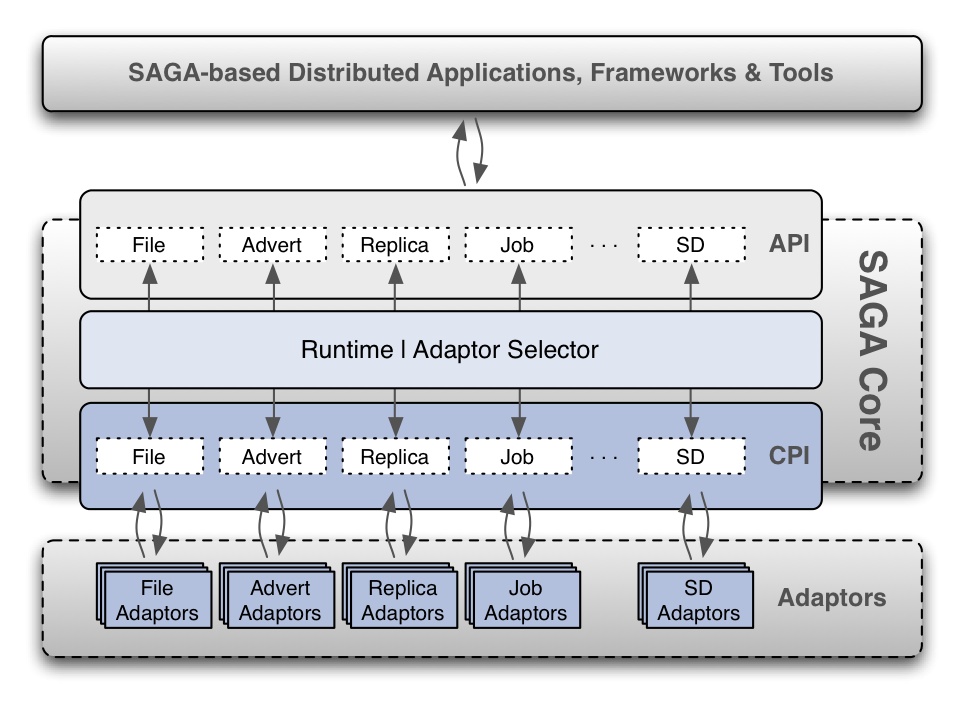
\includegraphics[width=0.66\textwidth]{figures/saga-architecture-1.png}
\caption{\textbf{SAGA Overview: } SAGA is an OGF technical
 specification that provides a common interface to heterogeneous DCI
 -- hitherto typically Grid systems. The implementation of the
 SAGA\cite{saga_url} specification consists of a high-level {\it
  API}, the SAGA {\it Engine} providing that API, and backend,
 system-specific {\it Adaptors}. The engine is a lightweight,
 highly-configurable dynamic library that manages call dispatching
 and the dynamic runtime loading of the middleware adaptors. Each of
 these adaptors implements the functionality of a specific functional
 package (e.g., job adaptors, file adaptors) for a specific
 middleware system. Adaptors are also realized as dynamic libraries.}
 \label{fig:saga-overview}
\end{figure}

A SAGA implementation consists of a high-level API, the SAGA
Engine providing that API, and backend, middleware/systems specific
adaptors. Each of these adaptors implements the functionality of
a functional package (e.g., job adaptors, file adaptors) for a
specific middleware system. The engine is a dynamic library that
manages call dispatching and the runtime loading of the middleware
adaptors. Adaptors are also realized as dynamic libraries. The SAGA
API has been used (in C++, Python and Java versions) to provide almost
complete coverage over nearly all grid and distributed computing
middleware/systems, including but not limited to Condor, Genesis,
Globus, UNICORE, LSF/PBS/Torque and Amazon EC2.

SAGA is currently used on production Cyberinfrastructure in several ways.
Admittedly the number of first-principle distributed applications developed is
low, but SAGA has been used to develop glue-code and tools that are
used to submit and marshal jobs \& data across and between
heterogeneous resources. Specifically, it has been used to support
multiple computational biology applications that use high-performance
and high-throughput molecular dynamics (MD) simulations.

% \jhanote{Someone please look up the macros as defined in the
%   pilot-star paper
%   \url{https://svn.cct.lsu.edu/repos/saga-projects/papers/troy/pstar/pstar-hpdc2012-acm.tex}
%   define here too and then do a global replace/consistency check
%   please.}  \yyenote{This has NOT been done. At this point people will
%   just wikipedia pilot job and get to the page started by the condor
%   folks (and modified by you)}

\subsection{Support for Dynamic Execution: SAGA-based Pilot-Job}

HPDC infrastructure is by definition comprised of a set of resources
that is fluctuating -- growing, shrinking, changing in load and
capability. This is in contrast to a static resource utilization model
traditionally a characteristic of parallel and cluster computing. The
ability to utilize a dynamic resource pool is thus an important
attribute of any application that needs to utilize HPDC infrastructure
efficiently. Applications that support dynamic execution have the
ability to respond to a fluctuating resource pool, i.\,e., the set of
resources utilized at time (T), $T=0$ is not the same as $T>0$.
However, even for traditional high-performance/parallel applications,
the evolution or internal dynamics of an application may vary, thereby
changing the resource requirements. For example, different solvers,
adaptive algorithms and/or implementations, can also require
applications to utilize different set/amounts of resources. Thus, the
need to support dynamic execution is widespread for computational
science applications. In DARE, this is accomplished by building
execution patterns using the SAGA-based Pilot-Job.
 
A common approach for decoupling workload management and resource
scheduling, and thereby the dynamic fluctuations inherent in workloads
and resources, is the use of \emph{pilot-jobs (PJ)}. The PJ
abstraction is also a promising route to address additional
requirements of distributed scientific
applications~\cite{ko-efficient,bigjob_cloudcom10}, such as
application-level scheduling.
 
\begin{figure}[t]
 \centering
% 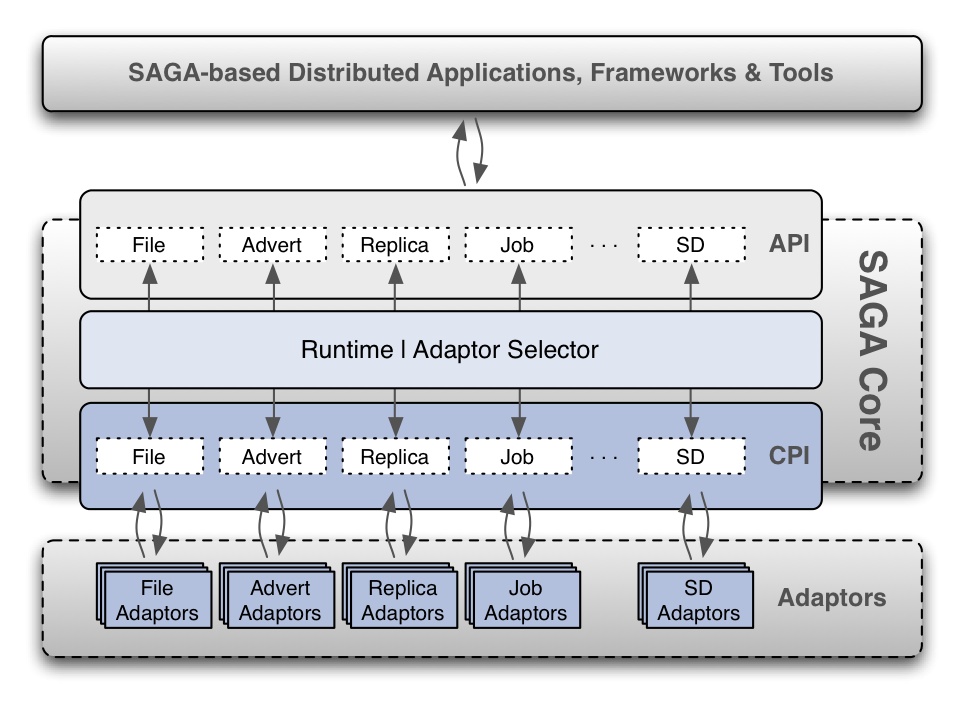
\includegraphics[width=0.48\textwidth]{figures/saga-architecture-1.png}
  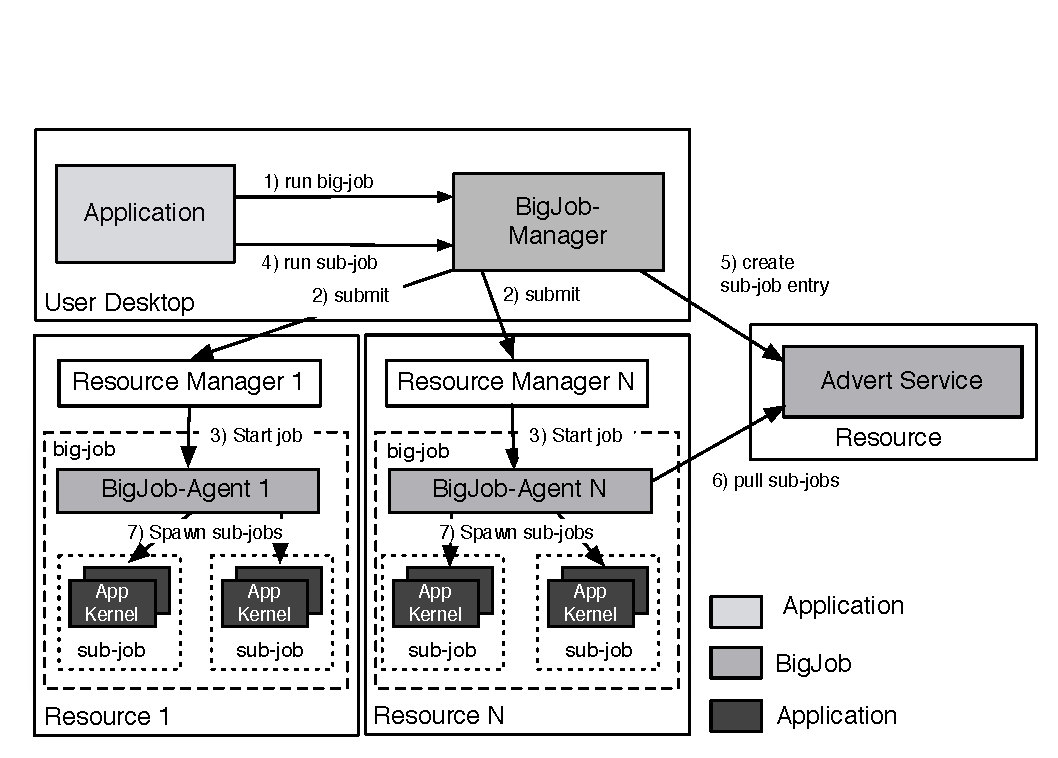
\includegraphics[width=0.48\textwidth]{figures/re_bigjob_interactions.pdf}
 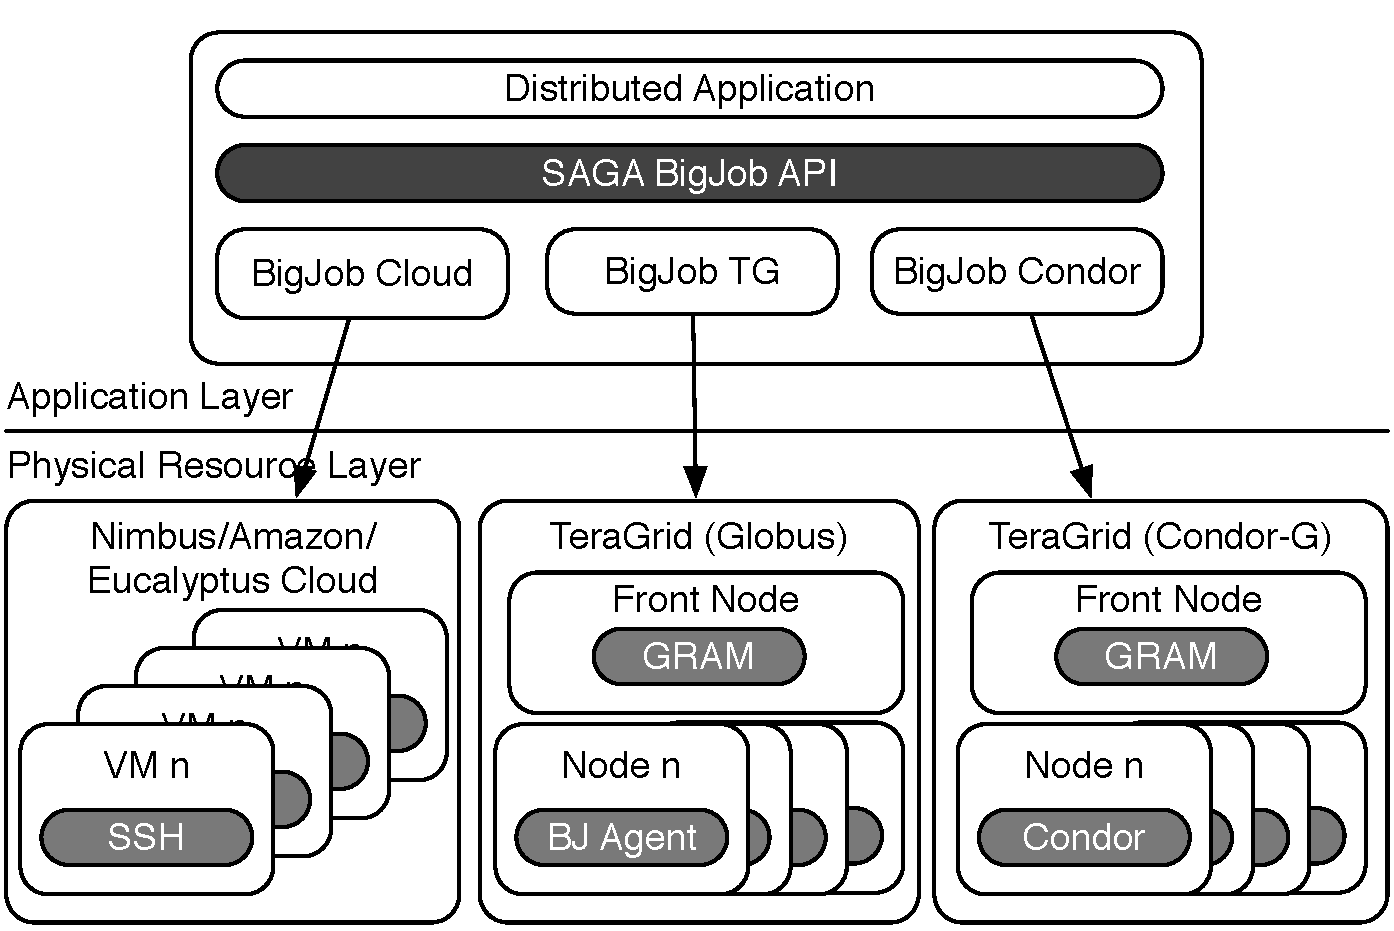
\includegraphics[width=0.48\textwidth]{figures/distributed_pilot_job.pdf}

    \caption{\textbf{BigJob Architecture:} The core of the
     framework, the BigJob-Manager orchestrates a set of
     pilots. Pilots are started using the SAGA Job API. The
     application submits work units, the so-called sub-jobs via the
     BigJob-Manager. Communication between the BJ-Manager and
     BJ-Agent is done via a shared data space, the Advert
     Service. The BJ-Agent is responsible for managing and
     monitoring sub-jobs. From
     Ref.~\cite{saga_bigjob_condor_cloud}}
    \label{fig:figures_re_bigjob_interactions}
\end{figure}

The SAGA-based pilot-job extends and generalizes the commonly used
Pilot-Job concept.  As a solid validation of the base standards and
abstractions that can be built upon SAGA, the SAGA-based pilot job has
enabled applications to use the same pilot-job API over disparate
resources. It has also provided advantages including scalability,
simplicity and extensibility. Similar advantages of scalability,
simplicity and extensibility are now available to Gateway developers
as a consequence of DARE – a SAGA-based library for developing Science
Gateways. A SAGA-based PilotJob, BigJob
(BJ)~\cite{bigjob_web,saga_bigjob_condor_cloud}, is a general-purpose
pilot-job framework. BigJob has been used to support various execution
patterns and execution workflows~\cite{async_repex11,saga-royalsoc}.
For example, SAGA-BigJob was used to execute scientific applications
categorized as embarrassingly parallel applications and loosely
coupled applications on scalable distributed
resources~\cite{ecmls_ccpe10, dare-ecmls11}.

Figure~\ref{fig:figures_re_bigjob_interactions} illustrates the
architecture of BJ. BJ utilizes a Master-Worker coordination model. The
BigJob-Manager is responsible for the orchestration of pilots, for the
binding of sub-jobs. For submission of the pilots, SAGA relies on the
SAGA Job API, and thus can be used in conjunction with different SAGA
adaptors, e.\,g.\ the Globus, the PBS, the Condor and the Amazon Web
Service adaptor. Each pilot initializes a so called BJ-agent. The
agent is responsible for gathering local information and for executing
tasks on its local resource. The SAGA Advert Service API is used for
communication between manager and agent. The Advert Service (AS)
exposes a shared data space that can be accessed by manager and agent,
which use the AS to realize a push/pull communication pattern.
The manager pushes a sub-job to the AS while the agents periodically pull
for new sub-jobs. Results and state updates are similarly pushed back from
the agent to the manager. Furthermore, BJ provides a pluggable
communication \& coordination layer and also supports alternative c\&c
systems, e.\,g.\ Redis~\cite{redis} and ZeroMQ~\cite{zmq}.

In many scenarios it is beneficial to utilize multiple resources,
e.\,g.\ to accelerate the time-to-completion or to provide resilience
to resource failures and/or unexpected delays (queue delays for
example).  BJ supports a wide range of application types, and is
usable over a broad range of infrastructures, i.\,e.\ it is
general-purpose and extensible
(Figure~\ref{fig:figures_re_bigjob_interactions}). In addition there
are specific BJ flavors for cloud resources such as Amazon EC2 and
Microsoft Azure that are capable of managing set of VMs, as well as a
BJ with a Condor-G based backend.  BJ supports dynamic resource
additions/removals as well as late binding. The support of this
feature depends on the backend used. To support this feature on top of
various BigJob implementations that are by default restricted to
single resource use (e.\,g.\ BJ), the concept of a BigJob pool is
introduced. A BigJob pool consists of multiple BJs (each BigJob
managing one particular resource). An extensible scheduler is used for
dispatching work units to one of the BJs of the pool (late
binding). By default a FIFO scheduler is provided.

% All user side aspects of BJ can be provided to end-users
% in a science gateway through DARE. Science gateway developers can
% expose as little or as much of BigJob as needed to the end-user as
% well as expose functionality for users to create workflows. Some
% commonly used workflows have already been built into DARE. These are
% referred to as pattern-based execution models.


The use of pilot-jobs as the fundamental execution unit lies at the
heart of the dynamic execution capabilities that DARE
support. Application and application-workflow execution can be
dynamic: some decisions can be made at runtime that affect the
behavior of the simulation, the resource used, data moved and so on.

% As resource platforms, network capabilities and data repositories grow
% in size, number and vary in interface, the emergence of a unifying
% framework (SAGA) was inevitable. SAGA demonstrated the capability (and
% usefulness) of overcoming utilization issues associated with
% distributed compute and data resources, complex multi-level workflows
% and runtime decision making~\ref{saga_url}.

\subsection{DARE: An Extensible Middleware Framework}


% \subsubsection{DARE: Support for Dynamic Execution and Execution
%   Patterns}
% \jhanote{See Fig. 3: DARE is defined as L2 and L3: SAGA + SAGA-based
%  Pilot-Job + Patterns (MR) + L2 (Application Capabilities)}

%{\it Support for Patterns-based Execution:} 
% Although not all of these are fully developed, a large number of
% execution patterns are already supported, e.g, uncoupled and
% loosely-coupled ensembles, Master-Worker, MapReduce etc.

Two features that distinguish DARE, include support for a range of
(common) application execution patterns and their easy integration
both with applications (above) and range of HPDC infrastructure
(below). The second distinguishing feature of DARE is its
extensibility along two dimensions: along the horizontal
dimension, new features and support for new execution patterns can be
added. In the vertical direction, support for new infrastructure can
be added.  

There are several common execution scenarios required for multiple
life-sciences applications. These scenarios include launching
ensembles of simulations or pipelines consisting of application
execution followed by analysis.  These can repeat any number of times
and include data-management or analysis stages. We refer to these
common execution scenarios as {\it execution patterns}. The provide
general templates frequently used in life sciences applications, e.g.,
well known patterns such as MapReduce and Scatter-Gather. DARE also
supports launching of large ensembles of loosely-coupled or uncoupled
tasks.  DARE's support for these common patterns is generic, and thus
easily adaptable to many different applications (not necessarily life
sciences).  In section \S3 we will discuss some of the common patterns
available in DARE. The support for a patterns-based execution is a
useful and novel feature of DARE.

Figure~\ref{fig:dare-arch} shows a layered architecture of a DARE
based science gateway in levels L2 and L3. Level L2 provides the
application and application workflow support along with templates for
common pre-configured usage scenarios: stand-alone, pipeline of
multiple tools, dynamic pipeline and general workflow support. Level
L3 provides the the runtime mechanisms that manage the execution of
specific implementations of these patterns. In the next section, we
explore this architecture in greater detail.

\section{DARE-based Science Gateways: Inside the Layered Architecture}

\begin{figure}
 \centering
% 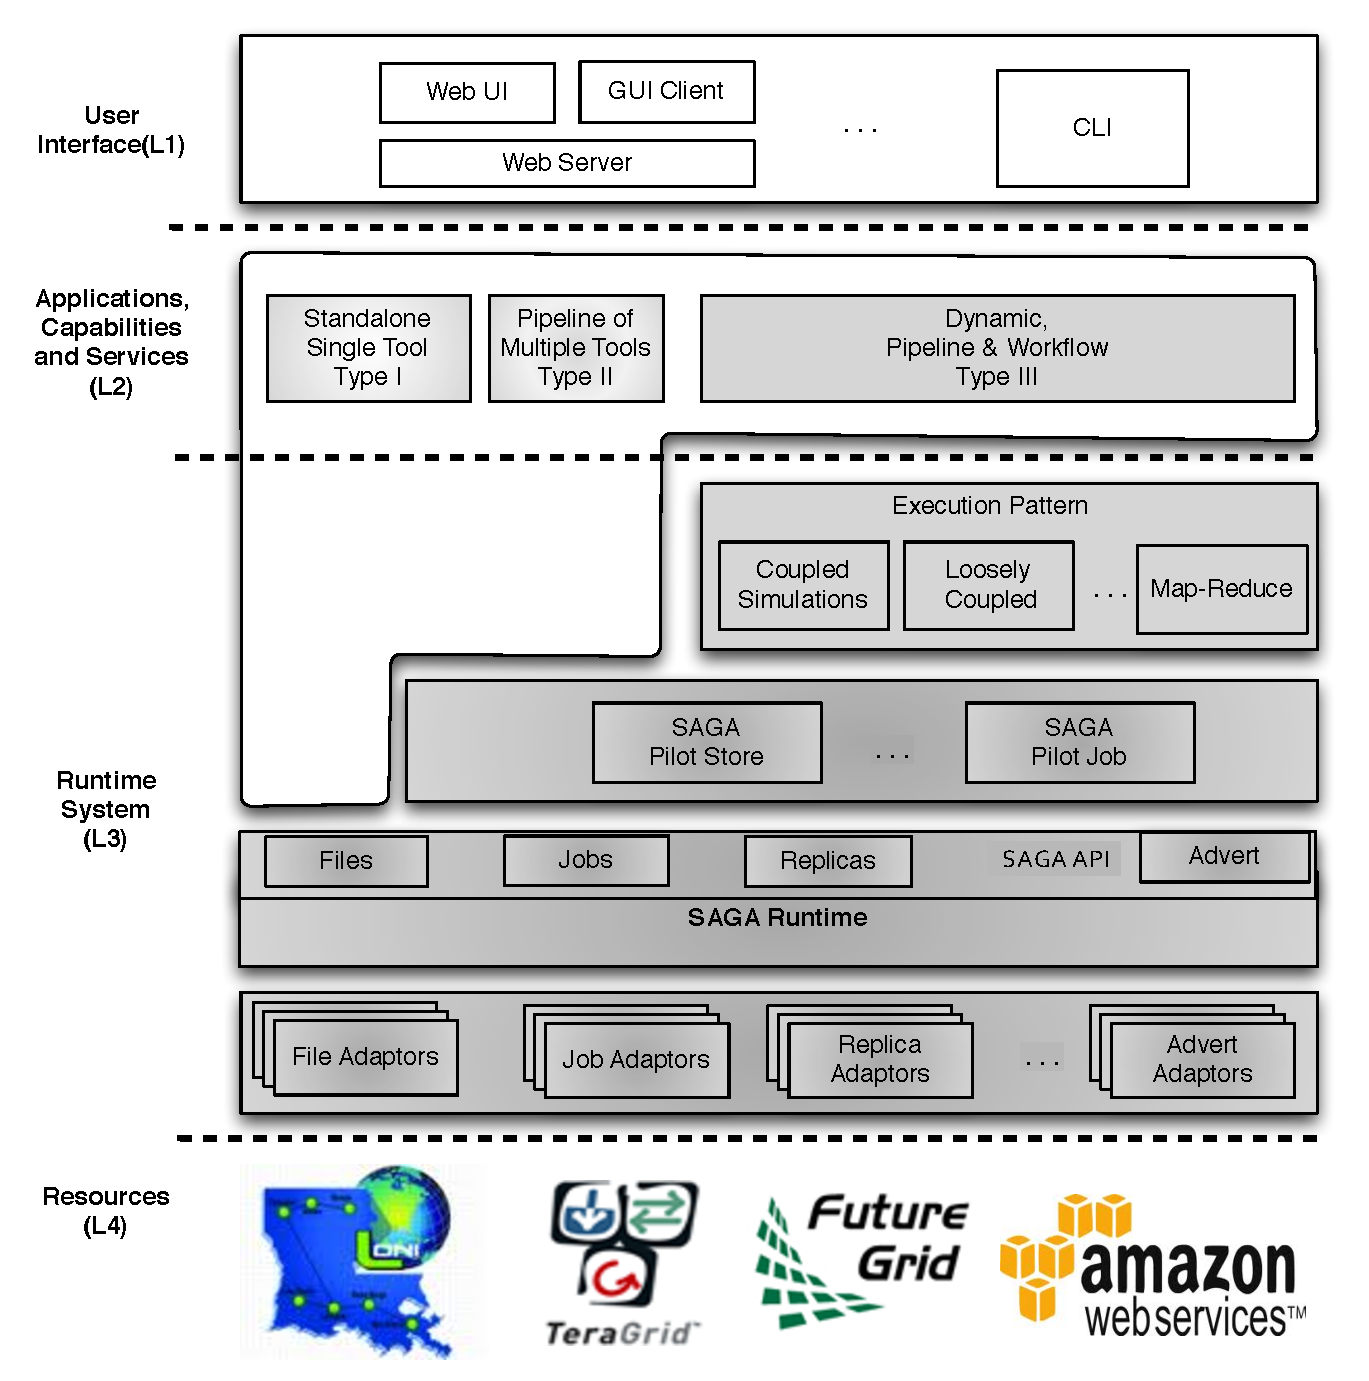
\includegraphics[scale=0.55]{figures/DARE-gateway-arch.pdf}
 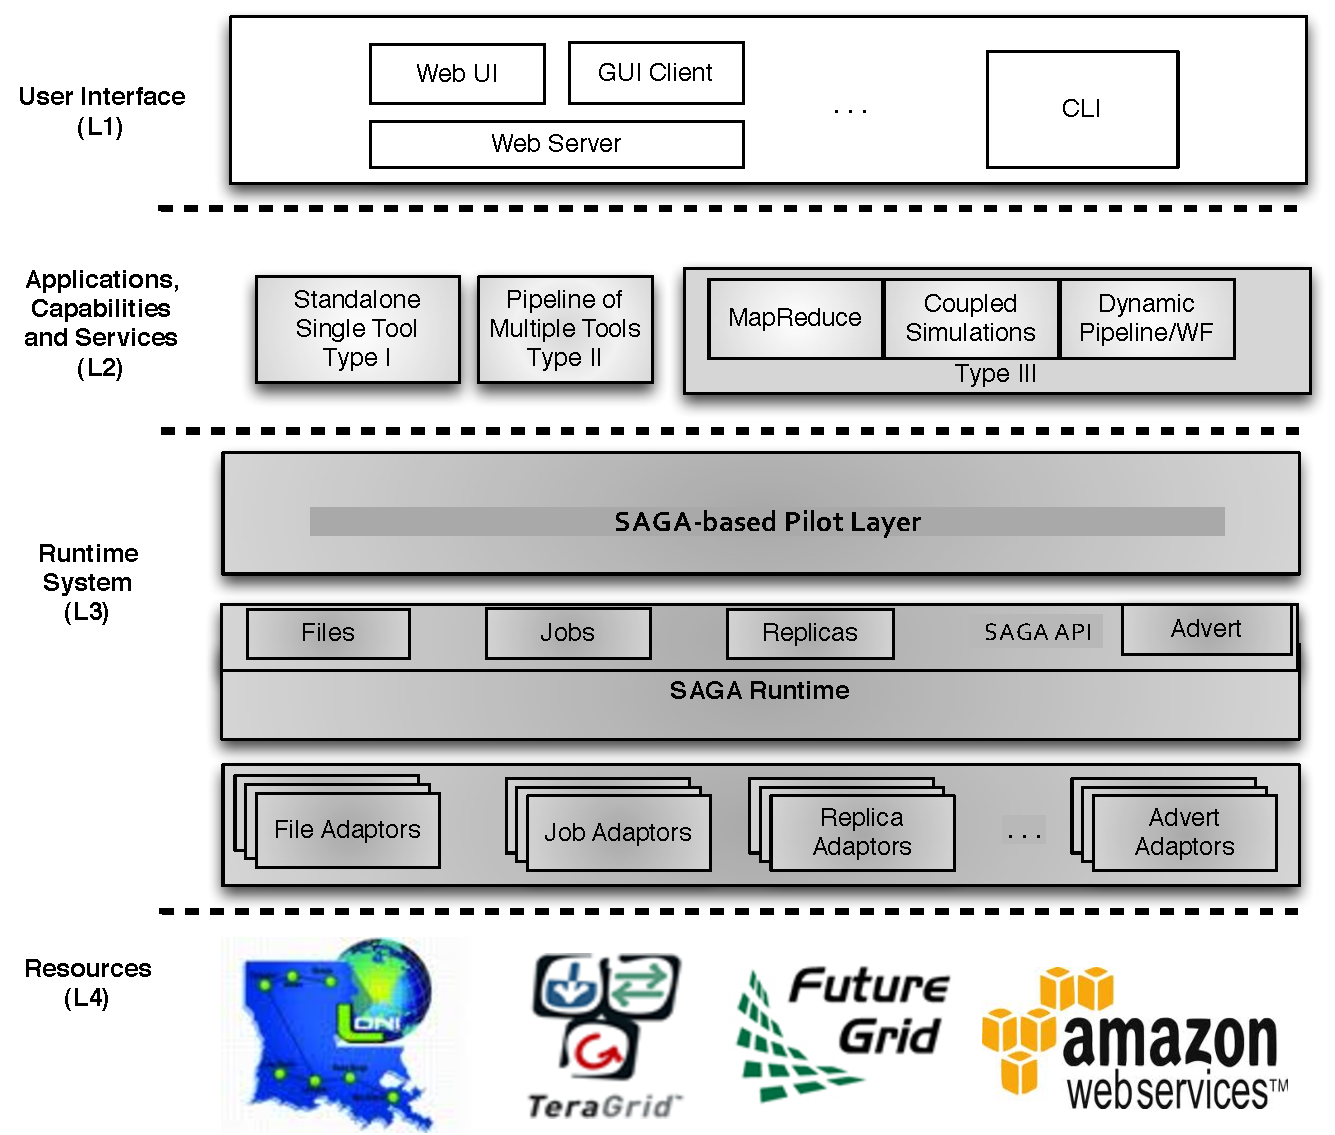
\includegraphics[scale=0.55]{figures/dare-middleware-arch.pdf}
 \caption{\small Overall architecture of a DARE-based gateway. L2 and
   L3 -- SAGA, SAGA-based pilot-jobs and support for application-level
   execution patterns, which are shaded in grey constitute the primary
   layers of DARE.}
 \label{fig:dare-arch}
\end{figure}

% , by glossing over details of function calls, 
% scripting language syntax and so on.

A typical gateway needs capabilties for everything from authentication
and authorization to the ability to submit user jobs, and data
management.  Ideally these capabilities are implemented without being
tied to specific resources, i.e., there is a role for a middleware
framework that integrates the usage of HPDC infrastructure with the
capabilities required to build user interface for science-gateways.
As illustrated in Fig.~\ref{fig:dare-arch}, DARE based science
gateways are typically organized into four levels: Levels L2 and L3,
are common to all gateways, and are decoupled from access level (L1)
and resource layer (L4). Development is therefore modular and
layered. Adding support for a new resource, for example OpenStack
based clouds in L4, is as simple as adding the required SAGA adaptors
in L3. No changes need to be made at L1 or L2. Similarly, adding more
execution patterns and workflows in L2 is decoupled from the runtime
system in L3 and the resources involved in L4.  We will not focus on
L1, other than to say that a combination of DARE-interfaces and
Pylons~\cite{pylons_website} (but could equally as well be Django) are
used as the building blocks to build user-interfaces that seamlessly
integrate with the rest of DARE and resulting functionality.


%\subsection{User Interface Level ($L1$)}
%\jhanote{This section is very unsmooth to read. Changes contexts/flow too many times} 

% Before we introduce the details about interfaces to DARE framework,  
% it is important to appreciate details about DARE and Pilot-API(P*-API) first. 
% The motivation behind DARE framework is to simplify the mechanism for
% the user to interact with different distributed resources for
% executing the complex workflows with various tools. 


\subsection{Applications, Capabilities and Services Level ($L2$)} 

The application layer (L2) contains the necessary infrastructure to
capture/express the logic necessary to create jobs of single
standalone applications, pipelines and the execution of non-linear
task dependencies.  These dependencies are expressed using the
DARE-interface alluded to, which is a customization of the
Pilot-API~\ref{pilot-api}. The Pilot-API provides a common access
layer to Pilot Job (Compute) and Pilot Data (File transfers)
frameworks over distributed production cyberinfrastructure, such as
XSEDE, OSG, EGI and FutureGrid.  While the Pilot-API hides the
complexity involved in the execution of tasks and file transfers on
distributed resources, DARE-layer provides a means for capturing the
dependency and the scheduling of different tasks.  Whilst, the same
scheduling can be achieved {\it directly} with just the Pilot-API,
DARE enables the auto-generation of scripts that implement these
capabilities, i.e., in other words, DARE provides a higher-level
capability on top of the Pilot-API.  This requires the simple
modification of necessary parameters in pre-exisiting templatized
configuration files.  This results in the creation of objects that are
in turn used by the Pilot-API by combining the user customized
configuration files.

These configuration files are carefully categorized into three
different types for simplicity and reusablity: (i) ConfType I: Holds
details about resources/machines for example job submission url, file
transfer url, authentication type, (ii) ConfType II: Provides
information about a tool, such as the location of a tool on different
resources and arguments that should be used for tools, and (iii)
ConfType III: Application instance specific information like location
of input files, which series of tools (ConfType II) to use and
resources as well as their size, wall time (ConfType I) etc.  Using
the information provided in the configuration files, DARE-level parses
the scheduling of tasks, via the creation of objects.  Furthermore,
the tasks and input/output files will be distributed over different
machines and need to be tracked.  DARE supports simple dependenceis
between tasks as managed via the Pilot-API.



% Before a task is submitted to the Pilot-API it
% should check for the status of its dependent task\cite{dare-wiki}. This
% automated scheduling feature of DARE is very helpful when the user
% has multiple tools in the pipeline for execution where the output
% files of one step become the input files for the next.

% Another important feature integrated into DARE is the ability to
% update the recent status of the job to a specified database.  


% Different
% DARE-Gateways have different web forms and workflow behind them.  


% Most Gateways commonly contain a well defined problem set where user
% want to just push a submit button with some minor changes in input
% files and tools.

% Pylons project is a collection of Python based web frameworks that
% are lightweight and easy to use. Pylons uses the common
% Model-Viewer-Controller design pattern and is written in Python.

% The DARE-Gateways web server is built using
% Pylon web framework.


These configuration file (ConfType II, ConfType III) are combinted to
provide three categories of patterns available to users: Types I, II
and III.  Type I is the simple, standalone tool.  Type II is a linear
pipeline of tools and type III includes non-linear tasks dependencies,
as well as complex interactions between them.  The Type I/II/III
classification also provides a natural and convenient breakdown of
available services, and was validated by its early applicability and
usability for life-sciences applications.
Table~\ref{table:three-type-service} shows some of the common life
sciences applications currently being used and their respective
pattern types. All of these applications can be used independently as
standalone Type I services.


% \jhanote{Please structure the discussion with some flow.  Define
%   what, then how!} \jhanote{what are these configurations of?}
% \jhanote{I still don't understand how one can instantiate an API?}
% \jhanote{Difference between DARE-API and what? Unclear...}
% \jhanote{P* undefined!?}  DARE-API is available for user
% installation and one can interact with DARE using the command line
% executable which comes with its installation.  DARE-API needs three
% key input configuration files which are necessary to execute a
% workflow on distributed machines.  Key features of DARE-API include
% a command line interface, generating the necessary objects required
% by the P-* API (Pilot data and Pilot Job) by combining user
% customized configuration files.  \jhanote{feature of what --
%   DARE-API or Pilot-API? Why can't we just use Pilot-API?}  DARE-API
% generate objects including resource, compute and file transfers
% information by the combination of different configuration files and
% submits them to P*-API.  \jhanote{Isn't that a usage mode of an API
%   rather than a different API?}  \jhanote{what is a DARE-API
%   workflow? Do you mean a workflow written using DARE-API?}
% \jhanote{What does this mean? How can an API have an executable?}
% \jhanote{How do you instantiate an API so as to execute a workflow!}
% \jhanote{BTW, its the Pilot-API} \jhanote{Not sure what the above is
%   trying to say}

%\jhanote{what is a pattern? Has that been defined?}  
% \jhanote{I do not know what ``.. is a necessary abstraction over the actual runtime systems'' means}


% Before understanding the details about applications layer it is
% important to know about the roles of different configurations
% files introduced earlier.


% During the DARE's runtime first it loads ConfType III after that it
% loads various ConfType I, ConfType II based on the location specified
% in ConfType III.

% DARE framework's scheduling mechanism entirely depends on the
% parameters in ConfType III. For example, there are two tools (Tool A,
% Tool B) for which Tool B's input files are dependent on Tool A's
% output file and wants to execute on distributed resources. All that is
% needed, is the modification of a parameter in a ConfType III
% file. DARE scheduling system waits until all the Tool A's jobs are
% completely finished and then submits Tool B's jobs. And this can get
% complicated as the number tools grow.

% A combination of early life sciences focus and gradual development led
% to this categorization.


\begin{table}[!h]
\centering
\begin{tabular}{| l | l | l | l |} \hline \rowcolor[rgb]{0.8,0.8,0.8} &
Type I & Type II & Type III \\ Description & Standalone & Pipeline & Dynamic  Workflows\\ 
& Single Tool & or Multiple Tools & \\\hline 
% Target Tool Modification & Not Needed &
% Not Needed & Minimally Needed \\ \hline Scientific Workflow & Not Needed & Useful but Not Necessarily &
% Needed \\ \hline 
NGS Example & BFast, BWA, & MACS, TopHat-Fusion, &  Novel Service for 
 \\
 & Bowtie, ABySS & TRANS-ABySS, Hydra & RNA-Seq \\
\hline
\end{tabular}
\caption{Comparison of three kinds of services provided by the
 DARE-based gateways. The lower row provides specific examples of
 services implemented for NGS analytics as part of DARE-NGS.}
\label{table:three-type-service}
\end{table}


In general, a program developed as a single standalone application needs
less effort. These are typically provided as Type I service. In contrast,
Type II services are built by incorporating different individual
tools/applications, and linked so that the output of one is
pre-determined as the input of another, i.e., provided as pipelines.
Making a pipeline available as Type II services provides
two major advantages: availability of multiple tools that are used in
conjunction with each other in one location, and the enhanced
capability to utilize scalable resources such as TG/XSEDE and other
HPC and Cloud resources.

On the other hand, Type III services aim to support more complex
service, both in the type of workflows supported as well as more
sophisticated execution like the input file changes dynamically from
job to job. In contrast Type I and Type II services aim to serve
stand-alone and pipelined tools with advanced cyberinfrastructure
capabilities, scalable production infrastructure and integrative
efficient pipelines. They are however limited to static execution:
once the job submission scripts are in, nothing can be changed.  Type
III workflows are fully customizable and extensible whereas Type II
workflows are predefined and used as is.  The specific resources that
are utilized in the execution phase are determined dynamically --
either through delayed binding or are refined/optimized after the
initial resource assignment.

There are two interfaces to access DARE functionality: DARE-Wrapper
and DARE-Gateways.  DARE-Wrapper provides a simple command line tool
named ``\texttt{dare-run}'' , which takes a configuration file as an
argument and initiates function calls to DARE passing out the given
configuration file. DARE-Gateways is a web interface, which provides a
simple user interaction for the services applications level L2.

DARE uses SAGA to support job-state monitoring and notification; this
capability is used to update status of submitted jobs. After
submission these parameters will be stored in a database. Further user
can look the status of the job that he has submitted and download the
output files once its done.  A job monitoring thread is an important
component inside DARE-Gateways.  Its functionality is to continuously
poll the database for new tasks, and whenever it finds a new job it
spawns a job after it creates the necessary configuration files.
Further, connecting the web interface to the server-side DARE services
is made simple with job monitoring thread.  DARE uses
Pylons~\cite{pylons_website}, and in the process out-sources
authentication, database creation/management, and data
storage/retrieval.  The database inside DARE-Gateways is defined in
such a way it could hold information about the job submitted by the
user as well as the user authentication information for login and
registration.

\subsection{Runtime System Level ($L3$) and its Integration with
  ($L4$)}

The DARE framework provides the two main features required for science
gateway development: task management and data management.  These
features are critical for distributed heterogeneous resource
utilization. As mentioned earlier, the pilot job abstraction,
SAGA-BigJob, has been successfully developed for distributed task
management and integrated into the current DARE framework as a key
component.  L3 represents the core of the DARE framework. In a
nutshell, it integrates the application-level capabilities (L2,
support for Type I/II/III services) with the HPDC infrastructure
(resources/L4) layer. The DARE runtime level in turn achieves this via
a critical dependence on SAGA. The challenges in building a scalable
distributed gateway are greatly mitigated by SAGA and/or SAGA-based
frameworks. The SAGA-runtime system has the responsibility to make
middleware specific dispatches.  The SAGA-BigJob (Pilot Job) supports
dynamic configuration changes, thus it is relatively easy to optimize
the usage of target resources for a given computational workload and
their execution characteristics. Examples include embarrassingly
parallel, loosely-coupled, or even multiple instances of
tightly-coupled applications. Thus once the desired configuration has
been determined, a gateway developer can easily construct an optimized
runtime environment for a given target application capable of
utilizing distributed resources without any application or
infrastructure refactoring.

SAGA and SAGA-based frameworks enable distributed scale-out across
multiple production grade resources. These production grade resources
include grids of large systems such as Ranger, Kraken and Lonestar as
well as HPC clouds on FutureGrid and vendor solutions such as Amazon's
EC2. A basic design principle that the runtime system adheres to is
future-proofing through extensibility and abstraction. When adding a
new computing platform, only a small amount of code has to be written
as a SAGA adaptor to enable access to that platform.

To cement support for different resources in L4, SAGA was deployed
publicly on XSEDE. The installations are available for anyone and
everyone to use: no private or shared accounts, no special
permissions. Ranger, Lonestar, Kraken, Trestles, Steele as well as
most FutureGrid machines have SAGA installations that are maintained
and kept up to date by the SAGA team and supporting XSEDE
personnel. Furthermore, several virtual machine images with SAGA
installations are available publicly on EC2. Any science gateway
developer can in principle and practice use these installations for
their DARE based science gateway.

Furthermore, it is important to consider data movement requirements,
since the movement of large data sets (input, output, and temporary
files) is a major challenge.  For data management, SAGA-BigData (Pilot
Data)~\cite{pstar12} is being actively developed in parallel to BigJob
which is used in DARE as well.  We have recently analyzed the
date-volumes that need to be moved around, and demonstrated some of
the challenges and solutions for BFAST~\cite{dare-ecmls11}, an NGS
application prototype.  As we will discuss in \S4, typical
data-volumes for NGS applications can easily exceed 100GB;
data-movement services need to and can managed these volumes. The
current implementation of DARE relies on data movement solutions
provided by BigData(Pilot Data).  It is worth noting that SAGA
supports different transfer protocols along with data-intensive
programming models such as MapReduce.  At the moment, GridFTP, scp and
Globus-online are used as the primary protocols for data transfer.
Thanks to the dynamic adaptor loading mechanism, SAGA can provide
these execution patterns for emerging data intensive computing
infrastructure such as
clouds~\cite{bigjob_cloudcom10,saga_bigjob_condor_cloud}.


% A Globus-Online adaptor is being developed for SAGA.
% The concept is to provide web-users with an interface very
% similar to Globus-Online, complete with scheduled file transfers,
% third party transfers, pause/resume, bandwidth caps, error detection
% and notification and routing options. A global file index is also
% being developed to catalog input data sets and their locations, along
% with locations of archived data around XSEDE resources.


\section{EXAMPLES OF DARE-BASED GATEWAYS FOR LIFE SCIENCES}

In spite of fundamental limitations on the precision of the data,
amongst the many indicators of the importance of computing in the life
sciences, is the fact that for most production distributed
cyberinfrastructure, the proportion of resources devoted to the life
sciences is already more than any discipline and the usage seems to be
increasing. This is valid whether measured by number of cycles
consumed, users or allocations.  However, this rise has been dominated
by a few well-established domains, such as large-scale Molecular
Dynamics (MD) simulations, and phylogenetics.  The former has
benefited from the availability of multiple community codes, tailored
to effectively utilize the computing infrastructure, thus enabling
easy uptake/usage amongst the scientific community.  The need for
large-scale distributed parallel execution for other areas of
life-science applications is growing.  This need is highlighted by
Next-Generation DNA Sequencing (NGS) which requires significant levels
of computing coupled with large-scale management and storage.  To
reinforce the importance of this point, the first DARE-based gateway
we present is DARE-NGS, and discuss scientific advantages that arise
from the DARE-based gateways, as a form of validation of concept and
implementation.

% Reinforcing this point, the first DARE-based gateway we present is
% DARE-NGS to support NGS analytics. We also present scientific
% advantages that arise from the DARE-based gateways.


% A specific example highlighting trends and advances in experimental
%  techniques producing large scale data sets with their high-throughput
%  methods, is provided by Next-Generation DNA Sequencing (NGS), and its
%  associated challenge of increasing computational sophistication
%  required in the gathering, management, and the analysis of derived
%  and produced data

\subsection{DARE-NGS}


\begin{table}
\centering
\scriptsize
 \begin{tabular}{|c|c|c|c|c|c|c|} 
 \hline 
Genome & Index         & Resource    & \# of & \# of &   \# of         &	TTC  \\
  Type               & File (GB)        & &Cores &   nodes &  VMs&  (sec)\\  
  \hline
 BG &0.435& R&	64 &4&-	&1067 \\
\hline                  
BG &0.435& QB	&	64& 8&-	&719 \\
\hline
 BG &0.435&R/QB	&	32/32 &2/4& -&919 \\
\hline
 BG &0.435& FG &	64 &-&8	&712 \\
\hline
 BG &0.435 &  R/QB/ &	24/24/& 2/3 & 3 &1022\\
 & & FG& 24 &&&\\
\hline
\hline
Chr &1.9& R	&	64& 4 &-&1145 \\
\hline
Chr &1.9& QB	&	64&8&-	&924 \\
\hline
Chr &1.9& R/QB	&	32/32& 4/2&	-&1170 \\
%\hline
%HG18-Chr21 &1.9& FG	&	64	& \\
%\hline
%HG18-Chr21 &1.9& R/QB/FG	&	24(2),24(3),	& \\
%&& 	 &24(3)&\\
\hline
\hline
HG &127& R	&	256 & 16 &-	&9586\\
%\hline
%HG &127& QB	&	256 &32 &-	& \\
\hline
HG &127& R/QB	&	128/128&8/16 & -&7582 \\
\hline
\end{tabular}
\caption{
  Comparison of Time to Completion (TTC) required for the NGS data
  mapping calculations using BFAST (match step) using DARE-NGS. 
  Three genome types,
  HG18 (HG), HG18-Chr21(Chr), B. Glumae(BG) represent a human genome,
  chromosome 21 of HG18, and the genome of a microbe Burkerholderia
  Glumae. Three compute resources are Ranger (R), QueenBee (QB), and
  FutureGrid  Eucalyptus Cloud on Sierra (FG), respectively. The
  number of tasks for carrying out the required mapping calculation is
  30 (135MB) for B. Glumae and 32 (169MB)for HG18 and HG18-Chr21. VM stands for virtual machines
}

  \label{table:NGS-Distributed} 
\end{table}

The DARE-NGS gateway % (\url{http://dare.cct.lsu.edu/gateways/ngs})
is one of our signature gateways built upon the DARE framework and focusing on
Next-Generation Sequencing data analytics and downstream analysis; it
currently supports essential computational tasks for NGS data analytics, including multiple mapping tools such as  BFAST, BWA, and Bowtie and pipelines for RNA-Seq and ChIP-Seq\cite{mardis2008-arghg,ecmls_ccpe10}. Mapping (alignment) is the first step, along with de novo assembly, in scientific discovery employing NGS sequencing-based protocols, i.e., the whole genome resequencing, RNA-Seq, and ChIP-Seq.  And the offering of available services and the capacity to handle large volume of data is still growing.

In the previous work~\cite{dare-ecmls11}, using DARE-NGS, we have analyzed the performance of BFAST, a mapping program representing the latest generation of mappers.  The tool stands out with its development goal for providing high sensitivity in analysis, whereas the design objective of most other popular mappers has been to achieve computational efficiency, i.e. less memory, computing time, computing resource, etc.  In fact, the computational complexity of the analysis (e.g. mapping) depends upon various elements such as the size and complexity of the reference genome and the data-size of short reads, but mostly algorithms.  We characterized the computational requirements, I/O bottlenecks and degree of concurrency with BFAST in Ref.~\cite{dare-ecmls11}, and concluded that an efficient, scalable and extensible analytical approach must be supported by any framework supporting NGS-analytics.

An examination of various execution scenarios with multiple
grid and cloud resources was conducted and a part of obtained results are presented in Table~\ref{table:NGS-Distributed}.  Not surprisingly, challenges are more involved than effective distribution of computational tasks across multiple, heterogeneous
resources; there is the need to manage large data movement and
storage.  Specifically, managing large-data volumes on FutureGrid
clouds required the Walrus data storage system\cite{walrusurl}, however access to Walrus through
%\jhanote{Sharath please  provide reference to Walrus}
multiple VM's often failed.  Such failures need to be managed, as
human genome mapping requires greater disk space than is often
available in many environments, including FutureGrid. Interestingly,
we overcame some disk space limitations, by implementing and
exploiting task-level concurrency.

% Nonetheless, gateway development should be flexible and
% agile for future changes in resources and computing environments.
% While this demonstrates the capability of DARE-NGS for utilizing HPC
% grids and cloud environments, 

Based upon the types of capabilities summarized in
Table~\ref{table:NGS-Distributed} and their seamless utilization of
HPC grids such as TG/XSEDE and Clouds as part of
FutureGrid\cite{dare-ecmls11}, DARE framework has thus been shown to
provide the required data and compute management capabilities for NGS
analytics and is thus an effective building block for science gateway
for sequencing data analytics and downstream analysis.  For
data-intensive computation such as NGS analytics, file transfer
processes are important for the total time-to-completion;
Table~\ref{table:NGS-Distributed-file} shows the measured transfer
time. Currently, DARE-NGS employ GridFTP as a default protocol on the
grids and SCP for FutureGrid Sierra Cloud.
Table~\ref{table:NGS-Distributed-file} highlights some data volumes
that typically need to be transferred with data analytics for DARE-NGS
with a model system (human genome).


 \begin{table}
\centering
 \small
 \begin{tabular}{|c|c|c|c|c|c|c|c|c|} 
 \hline  
 	          & LW to QB (s)  & LW to Ranger(s) \\
 \hline                       
Avg. Rate && \\
MB/s & 112.04 $\pm 2$ &	    24.7 $\pm 2$  \\
 \hline                       
Index File	FTT & 1133  &	    5131.3      \\        
 \hline                       
Raw 	 Exome FTT&80.3 & 363.6\\                  
 \hline                       
Processed Short-&    & \\
Reads FTT&34&153.9  \\
 \hline                       
\end{tabular}
\caption{Estimated File transfer times in seconds (FTT) with GridFTP
  between a local workstation (LW; machine named cyder located at
  LSU), QueenBee (QB), and Ranger for the Human Genome index files(127
  GB), exome data (9 GB) and processed Short Read files (3.8 GB).}

 \label{table:NGS-Distributed-file} 
\end{table}

\begin{figure}
 \centering
% \fbox{
% 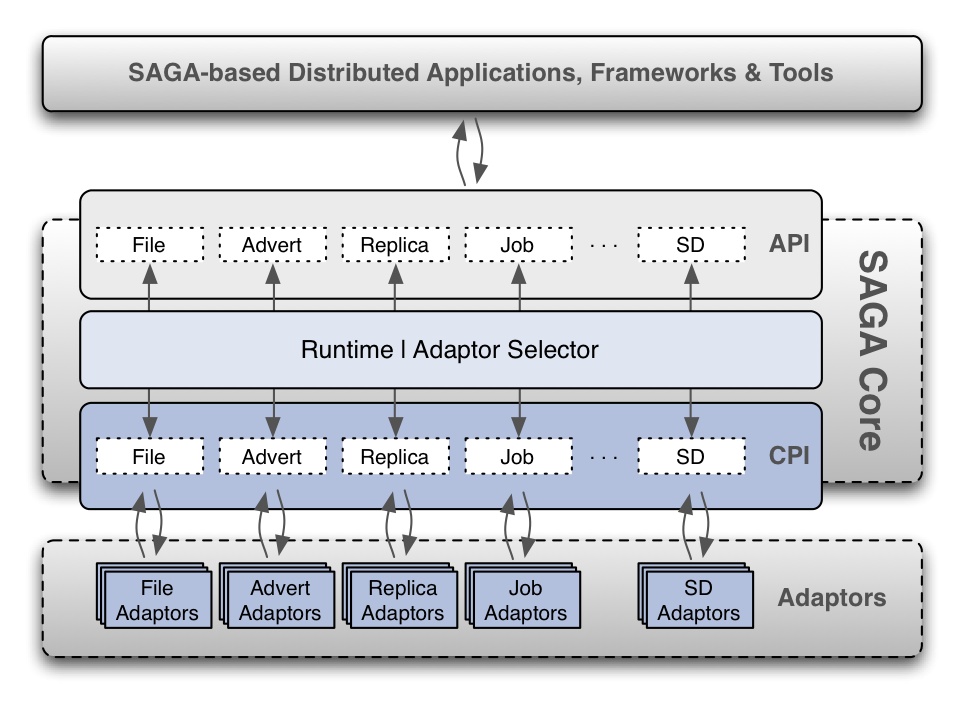
\includegraphics[width=0.66\textwidth]{figures/saga-architecture-1.png}
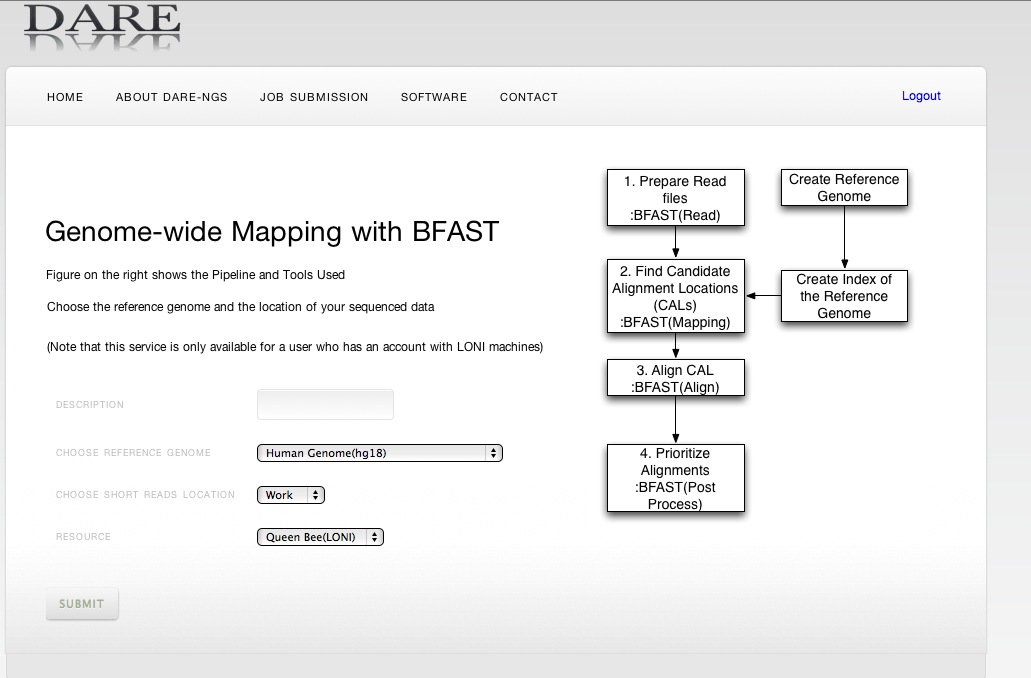
\includegraphics[width=0.5\textwidth]{figures/screenshot-ngs.png} \hspace{0.1in}
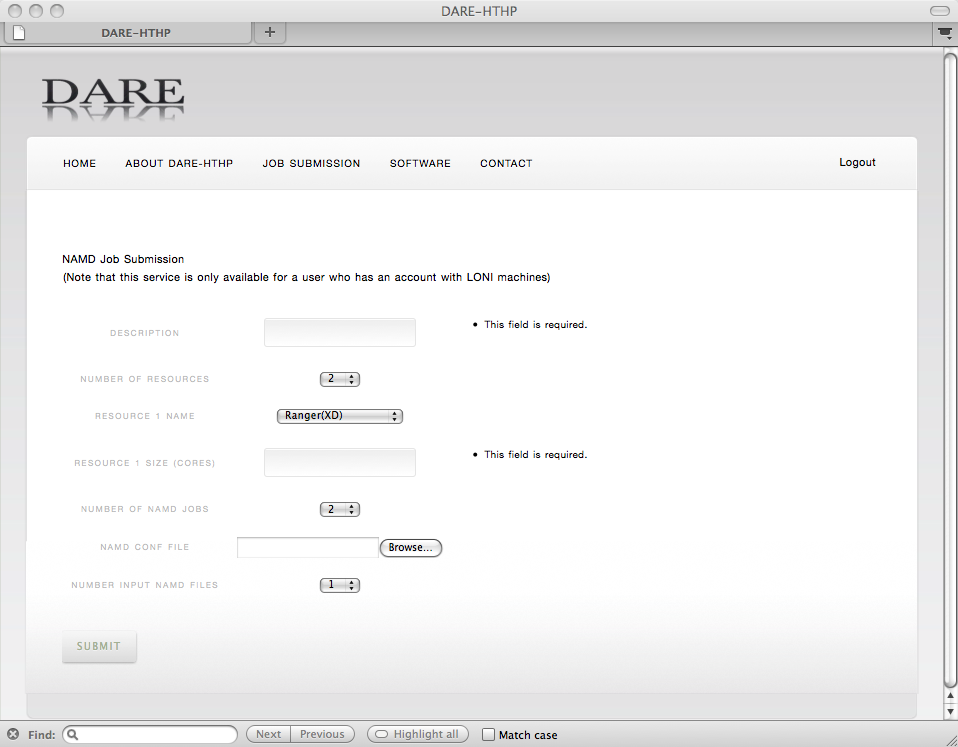
\includegraphics[width=0.42\textwidth]{figures/screenshot-hthp.png}
% }
\caption{\small (L) The User Interface of the DARE-NGS Gateway that
  utilizes DARE to execute BFAST (NGS) analytics. (R) NAMD job
  submission web page form through DARE-HTHP. Here, the form indicates
  the usage mode with multiple resources. The simple case with a
  single resource is default, and a user can expands the form by
  adding more resources as shown. DARE-HTHP and DARE-NGS can be
  accessed at: \url{http://dare.cct.lsu.edu} }
  \label{fig:NAMD2}
\end{figure}

% \yyenote{Following sentence needs clarification} An important
% challenge in modern biomolecular simulations, that has received
% insufficient attention is to get single long-running jobs completed,
% but managing and executing multiple instances of the same (or
% similar) physical system. There are multiple reasons behind this --
% ranging from higher accuracy to reduced time-to-solution. For
% example, multiple ensemble-member runs of the same physical system
% enable better sampling In some cases, such as free-energy
% calculations, multiple ensembles of the same system need to be
% utilized. And even where a single long-running simulation is
% required, thanks to algorithmic advances, such problems can be
% transformed into the more {\it tractable} problem of solving
% multiple shorter run simulations.

\subsection{DARE-HTHP}

In addition to long time simulations of a single large system, an
important challenge is the ability to run a large number of identical
copies (ensembles) of the same system. Ensemble-based simulations are
important for effective sampling and due to the low-level of coupling
between them, ensemble-based simulations are good candidates to
utilize distributed cyberinfrastructure.  The problem for the
practitioner is thus effectively marshaling thousands if not millions
of high-performance simulations on distributed cyberinfrastructure.

Thus fundamental support for an ensemble of simulations with the
following characters is required: (i) Usable on a range of underlying
distributed resources and independent of resource-specific middleware
and services (i.e. scale-across), (ii) Efficiently manage both
scale-up and scale-out of ensembles -- possibly scaling up to
tens-of-thousands, if not millions of ensembles, with varying degrees
of coupling, (iii) Effective for a range of physical model sizes --
from thousands of atoms to hundreds of thousands of atoms, (iv) All of
the above without being tied to a specific underlying MD kernel, (v)
Extensible and Interoperable with emerging computational platforms
such as clouds.

It is important to establish that the challenges of supporting
ensemble-based MD simulations are different from traditional workflows
(e.g, SCEC~\cite{scec-sc10}), where the emphasis is on coordination of
pre-ordered tasks; by contrast ensemble-based simulations need to be
designed to support the optimal scale-out and scale-up of tasks across
multiple machines. In other words, in the latter, the makespan has to
be reduced by executing as many tasks concurrently as possible,
whereas in traditional workflows the makespan has to be reduced by the
efficient scheduling and placement of ordered tasks.

In Ref.~\cite{bigjob-ccgrid12} the ability of an {\it interoperable}
and {\it extensible} pilot-job tool (BigJob), to support
high-throughput simulations of high-performance molecular dynamics
simulations across distributed supercomputing infrastructure was
assessed.  Specifically, a nucleosome positioning problem as an
exemplar was used, wherein we computed 336 independent trajectories of
20 ns each.  Each trajectory was further divided into twenty 1 ns long
simulation tasks. A single task required $\approx$ 42~MB of input, 9
hours of compute time on 32 cores, and generated 3.8~GB of data.  In
total 6,720 tasks (6.7 $ \mu $s ) and approximately 25~TB were
managed.  There is natural task-level concurrency, as these 6,720 can
be executed with 336-way task concurrency.  A scalable pilot-job
approach was used to successfully complete this workload on the
TeraGrid/XSEDE.

% Using NAMD 2.7, this project
% requires approximately 2 million hours of CPU time and could be
% completed in just over 1 month on a dedicated supercomputer containing
% 3,000 cores.  In practice even such a {\it modest} supercomputer is a
% shared resource and our experience suggests that a simple scheme to
% automatically batch queue the tasks, might require several years to
% complete the project.

Building upon these results, DARE-HTHP provides an extensible
middleware wrapper around SAGA-BigJob, as evidenced by results
presented in Table~\ref{table:HTHP-Distributed} (from
Ref.~\cite{ccpe11}), which establish that that DARE-HTHP support
ensembles of simulations across a range of HPDC infrastructure.

% \jkimnote{need the attention for the following. one or two sentence
%   summary would be desirable}

%When the user submits the job to run on Futuregrid cloud environment
%the input files are transferred to different VM's. The configuration
%files that are prepared in the Access/Application layer will be used
%to launch the DARE Framework which in turn starts/submits according
%to the job configuration provided by user across Grids and Clouds.

% To provide the capability to run jobs in cloud using DARE, we have
% prepared images which have SAGA and other required adaptors installed
% along with NAMD and MPI as well. These images are used to launch
% multiple VM's and job submission similar to grid
% environment. Furthermore, we are in a process of proving a capability
% where a user can upload their images, and DARE will transfer them to
% Eucalyptus cloud on Futuregrid and run on virtualized environment; it
% is also responsible for marshaling the VM's and tasks in these
% environments.

 \begin{table}
\centering
\small
 \begin{tabular}{|c|c|c|c|c|c|c|} 
 \hline 
 Number           & Resource    & \# of &  \# of     &     \# of     &	TTC  \\
of tasks                &     &  Cores    &nodes&   VMs  & (sec) \\  
\hline
8& R&	64	&4 & - &141\\
\hline                  
8& QB	&	64& 8 &	-&176 \\
\hline
4/4&R/QB	&	32/32 &2/4&-&151\\
\hline
8&FG	&	64(8) & - &8&414 \\
\hline
2/3/3&R/QB/FG	&32/24/24&2/3&	3 &384\\
\hline


\end{tabular}
\caption{Time to completion (TTC) for 8 tasks of NAMD (each running on 8 cores,
  irrespective of the underlying resources), run over different resources. The three
  compute resources are Ranger (R), QueenBee (QB), 
  and  FutureGrid  Eucalyptus Cloud on Sierra(FG), respectively. The
  data shows that DARE-HTHC has been run successively on Grids and
  Clouds concurrently.}
 \label{table:HTHP-Distributed} 
\end{table}

%\subsection{Other Examples}

In discussing DARE-NGS and DARE-HTHP, we have address how DARE has
been used to construct gateways, focusing on, (i) specific science
capabilities supported, (ii) demonstrating the use of a middleware
framework --- which serves as a common-layer to efficiently integrate
interface layer of a gateway with HPDC infrastructure, (iii) specific
problems solved, demonstrating the unique advantages of DARE-based
gateways for large scale compute-intensive as well as data-intensive
services are highlighted.  For example in DARE-NGS (one of the gateway
based on DARE-Gateways) a web form for CHiP-SEQ application where user
can choose parameters like reference genome, input files like control
and treat data and the mapping tools like BWA, Bowtie, and peak
calling tools like MACS, PeakSeq and submits the form.

Although the main uptake of DARE-based gateways has been for the
common scientific problems of NGS analytics and high-throughput MD
simulations, DARE is being used to construct gateways to address other
science requirements, viz. to study RNA folding and for large-scale
docking studies.  What is common amongst the ``family'' of gateways is
that they use the same DARE middleware framework, but each is
customized to support different science/application scenarios.


Here we outline briefly what needs to be done to extend DARE to
support other science/application scenarios: First step in creating a
custom Gateway is to create/modify configuration files (ConfType II)
for various tools in the targeted application and test the new
configuration with the DARE-Wrapper Next step is to create web forms
with necessary input fields and then a customize a function to convert
the user submitted web form into a configuration file (ConfType III).
Further, gateway developers can use DARE-Wrapper directly (Levels 2
and 3) and have their Gateways write DARE configuration files.  All
that is needed is to introduce the functionality to create/write a a
configuration file (ConfType III) with required parameters to run a
workflow and have this configuration file submitted while initiating
DARE-Wrapper. ConfType III holds the critical part of a job (instance
of application) as it has the information for that specific
application's instance. Since the same application may run faster or
slower based on the input file size, it is important to let the user
modify just before the runtime different tools like which resources
and their size based on input files for the job. Further user may also
want to change one of the various tools in the current workflow. These
minor changes can be achieved quickly just by changing a parameter
with a different ConfType II file in ConfType III.  There can be
multiple ConfType I files, ConfType II files for a single instance of
DARE-API but only one file with ConfType III.  DARE provides
pre-installed with some predefined configuration files which can be
modified, new configuration files created. Information about
additional parameters in configuration files can be found in the
DARE-wiki ~\cite{dare_api_web}.


% \jhanote{explain what is different between the gateways? Clearly the
%   DARE "middleware" is common but elaborate how starting from the
%   common middleware, the final Gateway was developed.}

% To support nc-RNA research and broadly for the community who is
% interested in the utilization of RNA structure prediction for their
% research goals and education purposes, we have been developing a
% gateway, DARE-RFOLD, with which a user is able to predict the Minimum
% Free Energy (MFE) secondary structure or an ensemble of structure
% sampled with a Boltzmann-weighted sampling scheme.

\section{Deploying DARE-based Gateways on TG/XSEDE}

% There are two ways in which DARE-based Gateways can be provided to
% users on XSEDE. The first involve the deployment of DARE-based
% Gateways on a ``static'' resource -- with fixed connectivity, number
% of users etc. The other involves the use of virtualized infrastructure
% to support the deployment of scalable gateway solutions. Static deployment
% is straightforward is less complex than virtualized deployments, 
% therefore we will concentrate on the latter and discuss the
% current and future data management capabilities.
% 
% \subsection{Deploying DARE-based Gateways Using Virtualized Resource}

Indiana's Quarry~\cite{quarry} has been used as a novel agile virtual hosting
service for DARE-based gateways. Quarry is a gateway hosting resource
consisting of
geographically distributed Dell AMD systems that provide persistent,
secure virtualization services. Typically gateways would run
statically on dedicated hardware that is not directly connected (or
affiliated) with XSEDE systems. With Quarry, gateways can be run from
gateway-developer run images hosted on an XSEDE resource with high
bandwidth connections to XSEDE HPC resources as well as data
repositories at TACC (Ranch), NCSA (Forge) and PSC (Albedo).

There are many advantages to agile virtualized gateway systems
including automatic nightly backups, quick restores (if re-deploying
after failure), reduced maintenance and so on. Furthermore, the
virtualized solution has low operational cost	s, high bandwidth and
excellent support. There is however a unique advantage to gateway
framework developers: the ability to bundle a VM image containing the
gateway framework for immediate, user-ready deployment. For DARE, the
bundled image will contain the basic framework along with
demonstration web interfaces: DARE-NGS and DARE-HTHP. If a third party
user (or gateway developer) wants to use DARE, all users have to do is
run the DARE image on Quarry and setup their credentials.

By contrast, most XSEDE (and formerly TeraGrid) science gateways ran
statically on hardware with low fault tolerance and custom web and
machine interfaces~\cite{xsedegateways}. In a
sense, this is a one-off custom solution that every group needing a
science gateway had to struggle with. Each of these gateways is a
unique installation running on user side resources with custom scripts
and more importantly custom interfaces to TeraGrid/XSEDE. This
complicates the deployment and utilization model of science gateways:
each gateway has to be a full ground-up development project and the
entire development and deployment burden is placed on the gateway
developers.

The deployment and utilization model for DARE shifts the development
and deployment effort so that regular users (not necessarily gateway
developers) can get a basic science gateway running in quick order
without much difficulty. With a basic understanding of gateways, a
user can start their own DARE VM on Quarry and customize the existing
building blocks and interfaces to their satisfaction. This reduces
XSEDE integration overhead, gateway development and deployment
overhead and unifies gateway infrastructure for many applications. It
is also important to note that other XSEDE sites are in the process of
deploying gateway hosting services similar to Quarry, and with VM
portability, DARE VM's can be ubiquitous on these resources as
well. Our expectation is to see science gateways as a generic but
customizable service available to users, complete with building blocks
in the form of ``canned'' virtual machine images.




% \subsection{Data Management in DARE-based Gateways}
% The DARE framework provides the two main features required
% for science gateway development: task management and data management.
% These features are critical for distributed heterogeneous resource
% utilization. As mentioned earlier, the pilot
% job abstraction, SAGA-BigJob, has been successfully developed for
% distributed task management and integrated into the current DARE
% framework as a key component. For data management, SAGA-BigData~\cite{pstar12} is
% being actively developed in parallel to BigJob.
% 
% The current implementation of DARE relies on data movement solutions
% provided by SAGA, namely GridFTP and SCP. A Globus-Online adaptor is
% being developed for SAGA, along with a DARE interface and a web
% API. The concept is to provide web-users with an interface very
% similar to Globus-Online, complete with scheduled file transfers,
% third party transfers, pause/resume, bandwidth caps, error detection
% and notification and routing options. A global file index is also
% being developed to catalog input data sets and their locations, along
% with locations of archived data around XSEDE resources. These DARE
% capabilities provide data movement and orchestration necessary for
% complex workflow support.
\section{Discussion}

The fact that DARE has been used to support four very different
science applications is testimony to the correct abstractions and
design objectives. In each case, DARE has facilitated the quick,
effective and scalable integration of the scientific logic associated
with the of a use-case/usage-mode (often implemented with python
scripts) with the underlying HPDC infrastructure/resources. Each of
these science applications and their usage-modes have been supported
via both {\it command-line} as well as {\it science gateway}
interfaces.

DARE supports the primary distributed application design objectives in
IDEAS~\cite{ideas} -- Interoperability, Dynamic execution,
Extensibility, Adaptivity and Scalability. One of these objectives,
scalability (in particular, scale-across), represents the ability to
utilize multiple resources; using these resources collectively has
many benefits, not least of which is the decrease in the
time-to-completion. As illustrated in
Table~\ref{table:NGS-Distributed}, DARE has been used to demonstrate
such performance improvements; specifically, where two large TG/XSEDE
systems -- QB and Ranger, were used for the match step in BFAST
pipeline. For the HTHP mode~\cite{bigjob-ccgrid12}, up to 24,192 cores
were utilized at the same time, 128 concurrent simulations were
managed (scale-out) and up to four different TeraGrid/XSEDE resources
used. Given the difference in middleware distributions, this also
demonstrates DARE's ability to support interoperability.

Functional and infrastructural extensibility are important
requirements for gateways; indeed, as we have shown, many levels of
extensibility are provided by DARE-based gateways. For example, the
SAGA-based approach which provide numerous adaptors to different
middleware, supports interoperability across different middleware
types; it is limited only by the availability of adaptors (SAGA has
relevant adaptors to multiple existing infrastructure including
clouds). The integration between L2 and L3 via different types of
services supported via a range of execution patterns and SAGA-based
pilot-abstractions, provide the flexibility to extend scientific
capability of a gateway, e.g., support of ensemble-based simulations
as a primitive ``execution unit''. Building upon the
Pilot-abstractions, DARE-based gateways also support extended
data-access patterns and coupled data-compute placement. Functional
extensibility is required for scientific inquiry; for example, with
DARE-RFOLD, we have provided a pipeline whereby the output from the
RNA secondary structure prediction was utilized for Riboswitch gene
annotation using structural information.

The experience of using DARE to support NGS analytics over a range of
input problem sizes, infrastructure and analytical problems, (as
illustrated by Table~\ref{table:NGS-Distributed}), indicate that
Science-Gateways for distributed data-intensive applications have a
set of unique challenges. For example, for NGS data alignment using
BFAST, not only does one need to determine the right distribution of
computational resources for the given tasks/problem at hand, but these
tasks need to be placed ``optimally'' so that data movement does not
become the bottleneck. DARE supports such {\it dynamic} resource
utilization and execution capabilities.


In conjunction with the ability to distribute tasks effectively, NGS
data alignment using BFAST, requires the ability to determine the
optimal task-level concurrency; this is often a function of how the
reference genome indexes are utilized for chunks of short read
data\cite{dare-ecmls11}. The design of the DARE framework supports
such application-level adaptivity, via support for flexible
composition of L2 services, and flexible execution patterns and
dynamic execution modes. As alluded to in \S~2.1, application-level
requirements must be matched by the runtime systems; here the runtime
systems such as SAGA-based pilot-jobs support application-level
adaptivity, e.g., change in task-level granularity, usage modes etc.
Other forms of adaptivity supported by the runtime systems that
DARE-based Gateways build upon, include different data-transfer
mechanisms -- varying from gridFTP, to reliable protocols and variants
thereof (such as GlobusOnline).

It is important to reiterate, that all of the objectives as captured
by IDEAS are provided by DARE using distributed computing community
{\it standards}. The lack of need to change interfaces and development
systems imparts a simplicity to the development process, i.e., SAGA is
the basis for the simplicity ensuing from the well defined interfaces
that supports multiple {\it standards} distributed functionality, as
well as higher-level abstractions, e.g., based on the underlying
SAGA-based API, via SAGA-BigJob a general purpose Pilot-Job
abstraction.

Finally, the new virtual machine image based deployment model on
Indiana's Data Quarry system enables rapid and hassle free
deployment. No hardware needs to be purchased, no backups arranged,
and web development. In due time, we expect to have popular content
management systems with DARE infrastructure available in images for
the entire community to use.

In summary, we have demonstrated via working examples, how providing
the right abstractions and easy integration with other components,
enables DARE-based gateways to support the effective and easy
development of science gateways for life-science applications that
support distributed applications, whilst adhering to the IDEAS
design-objectives. This includes advanced deployment modes and novel
data-intensive life-science applications that utilize emerging
distributed computing/data resources such as TG/XSEDE and cloud
environment contributes.

\section*{Acknowledgments}
This work is primarily supported and motivated by Grant Number
P20RR016456 from the NIH National Center For Research Resources. We
are grateful to Andre Luckow and Ole Weidner for their work for SAGA
and SAGA-BigJob development; we also thank Ole Weidner for a
constructive criticism of this manuscript and Andre Merzky for the
information about SAGA CSA deployment. Computing resources used for
this work were made possible via NSF TRAC award TG- MCB090174 and LONI
resources. This document was developed with support from the National
Science Foundation (NSF) under Grant No. 0910812 to Indiana University
for ``FutureGrid: An Experimental, High-Performance Grid
Test-bed.''. SJ would like to thank Dave Hart (SDSC) and Dan Katz
(Chicago) for helpful discussions. Last, but not least, we would like
to thank one of the anonymous reviewers for exceptionally useful and
insightful comments, which have greatly improved the paper. 


%\bibliographystyle{spbasic}   % basic style, author-year citations
%\bibliographystyle{spmpsci}   % mathematics and physical sciences
%\bibliographystyle{spphys}    % APS-like style for physics
%\bibliography{saga,tg11}
%\bibliographystyle{abbrv}

\bibliographystyle{unsrt}
\bibliography{radical_rutgers,jogc}
\end{document}


% \textbf{dare-run}: an executable that instantiates DARE with configuration files as input.
%
% \textbf{dare-manager}: a module inside the DARE package which carries
% out the execution imposed by dare-run and that is responsible for
% managing several functions such as preparing configuration files and
% detection of failure and successful termination.
% 
% \textbf{job}: a service invoked by a user via Gateway. It contains information about required tools. 
% 
% \textbf{pilot unit(PU)}: an object holding information about remote
% resources to be utilized. This is needed to launch pilot agents.
% Attributes for authentication, working directory, and data transfer
% urls are also assigned.
% 
% \textbf{step unit(SU)}: an object in DARE which holds the information
% about required computation and data transfers. For example, in the
% computation for a mapping with the bfast package, first we have to
% conduct an indexing task, then a mapping and then an alignment tasks.
% In DARE, we assign an indexing task as step 1, a mapping task as step
% 2 and an alignment task as step 3. step 1, an indexing step, has
% information about input files that is to be transferred to a remote
% resource(data unit) and a computational task that needs to be
% performed.

We have developed DARE-RFOLD and successfully utilized for non-coding
RNA research and also to serve the RNA structure prediction
community. Through DARE-RFOLD, users can run simulations to predict
the Minimum Free Energy (MFE) secondary structure or to obtain an
ensemble of structures sampled with a Boltzmann-weighted sampling
scheme.

Scientifically it is meaningful to integrated RFOLD with the
capabilities of DARE: investigation into the computational
requirements of RNA folding (or structure prediction) suggest that the
support of high-throughput computation for a large number of tasks on
heterogeneous distributed resources is beneficial for the exploration
of RNA folding energy landscape and structural characterization of
SAM-I riboswitch sequences. As shown in
Refs.~\cite{dare-ecmls11,ccpe11}, we demonstrated the DARE framework
and its ability to support many tasks of over multiple scales and
resources by effectively completing a total of 2910 tasks needed for
all known SAM-I RNA sequence family.

\subsubsection{DARE-DOCK}

\jhanote{Similar structure to DARE-RFOLD: How was the GW constructed
  using DARE. Was it all at the UI level?}

DARE-DOCK aims the basic virtual screening.  The current service with
the gateway supports the docking with a popular application,
Autodock\cite{autodock}.  Specifically, the docking calculation is
carried out with the Autodock-vina, which allows to utilize fine-grain
parallelism with multi-threading multi-core support.  By supporting a
service to run Autodock-vina, the gateway is able to carry out a very
effective execution of high-throughput docking with multiple resources
that is supported seamlessly by DARE.

%\begin{figure}
% \centering
%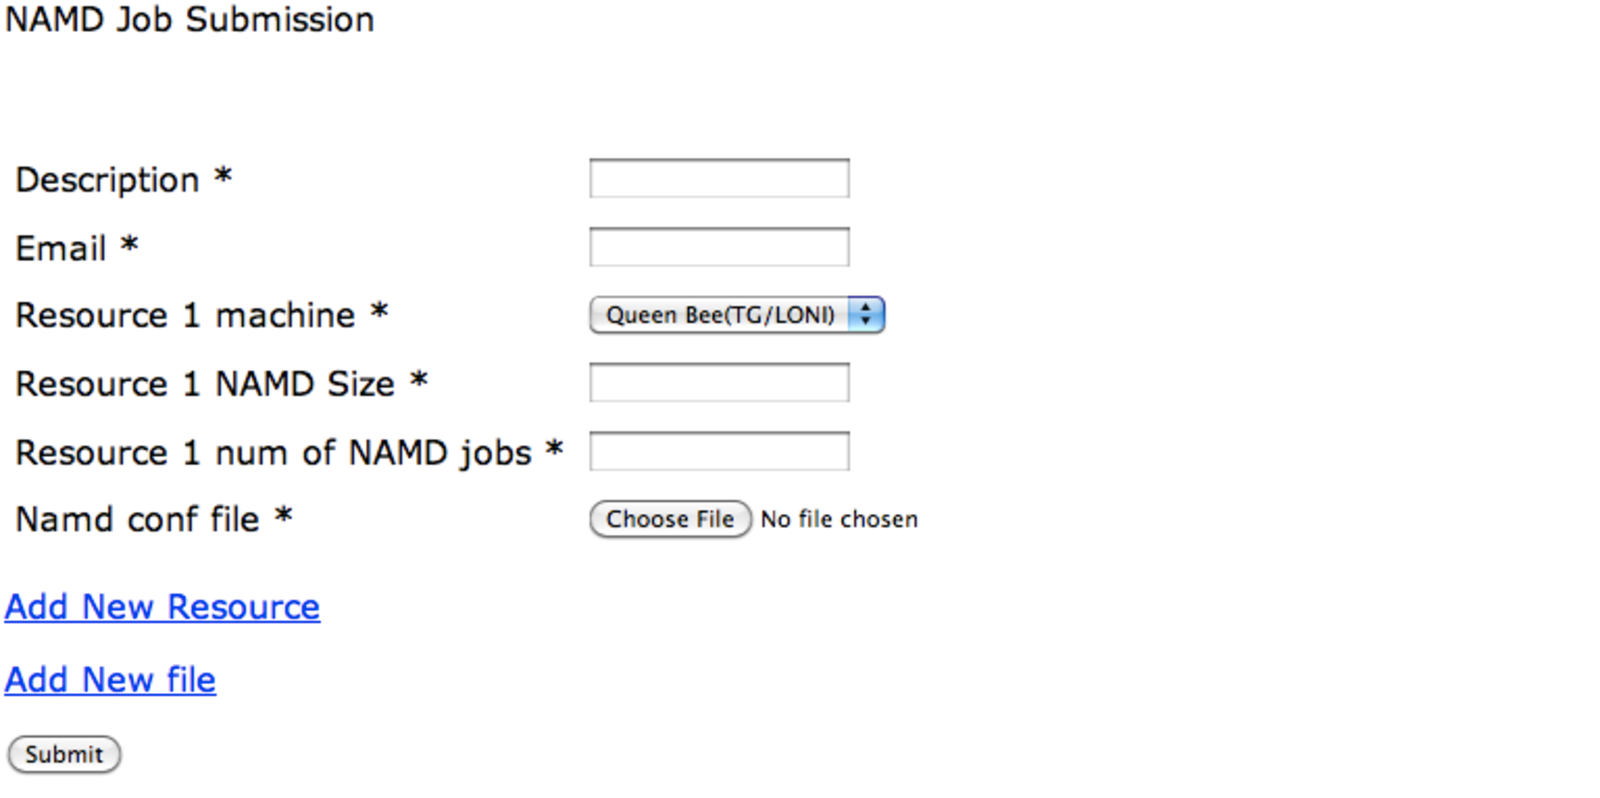
\includegraphics[scale=0.35]{figures/NAMD1.pdf}
%
%\caption{\small NAMD job submission web page form through DARE-HTHP} 
%\end{figure}

